\documentclass{vkr}
\usepackage[english, russian]{babel} % переносы
\usepackage{graphicx} % для вставки картинок
\graphicspath{{images/}} % путь к изображениям
\usepackage[hidelinks]{hyperref}
\usepackage{float} % определяет метод H для рисунка с переносом на следующую страницу, ели не помещается
\usepackage{pdflscape}
\addto{\captionsrussian}{\renewcommand{\refname}{СПИСОК ИСПОЛЬЗОВАННЫХ ИСТОЧНИКОВ}}
\usepackage{xltabular} % для вставки таблиц
\usepackage{makecell}
\renewcommand\theadfont{} % шрифт в /thead
\usepackage{array} % для определения новых типов столбцов таблиц
\newcolumntype{T}{>{\centering\arraybackslash}X} % новый тип столбца T - автоматическая ширина столбца с выравниванием по центру
\newcolumntype{R}{>{\raggedleft\arraybackslash}X} % новый тип столбца R - автоматическая ширина столбца с выравниванием по правому краю
\newcolumntype{C}[1]{>{\centering\let\newline\\\arraybackslash\hspace{0pt}}m{#1}} % новый тип столбца C - фиксированная ширина столбца с выравниванием по центру
\newcolumntype{r}[1]{>{\raggedleft\arraybackslash}p{#1}} % новый тип столбца r - фиксированная ширина столбца с выравниванием по правому краю
\newcommand{\centrow}{\centering\arraybackslash} % командой \centrow можно центрировать одну ячейку (заголовок) в столбце типа X или p, оставив в оcтальных ячейках другой тип выравнивания
\newcommand{\finishhead}{\endhead\hline\endlastfoot}
\newcommand{\continuecaption}[1]{\captionsetup{labelformat=empty} \caption[]{#1}\\ \hline }
\usepackage{etoolbox}
\AtBeginEnvironment{xltabular}{\refstepcounter{tablecnt}} % подсчет таблиц xltabular, обычные таблицы подсчитываются в классе

\usepackage[tableposition=top]{caption} % подпись таблицы вверху
\captionsetup{strut=off}
\setlength{\intextsep}{0pt} % Vertical space above & below [h] floats
\setlength{\textfloatsep}{0pt} % Vertical space below (above) [t] ([b]) floats
\DeclareCaptionLabelFormat{gostfigure}{Рисунок #2} %подпись рисунка
\DeclareCaptionLabelFormat{gosttable}{Таблица #2} %подпись таблицы
\DeclareCaptionLabelSeparator{gost}{~--~} %разделитель в рисунках и таблицах
\captionsetup{labelsep=gost}
\captionsetup[figure]{aboveskip=10pt,belowskip=4mm,justification=centering,labelformat=gostfigure} % настройка подписи рисунка
\captionsetup[table]{font={stretch=1.41},skip=0pt,belowskip=0pt,aboveskip=8.5pt,singlelinecheck=off,labelformat=gosttable} % настройка подписи таблицы

\setlength{\LTpre}{8mm} % отступ сверху таблицы
\setlength{\LTpost}{6mm} % отступ снизу таблицы

\usepackage{enumitem}
\setlist{nolistsep,wide=\parindent,itemindent=*} % отступы вокруг списков, выравнивание с учетом разделителя

\usepackage{color} %% это для отображения цвета в коде
\usepackage{listings} %% листинги кода
\setmonofont[Scale=0.7]{Verdana} % моноширный шрифт для листинга

\definecolor{codegreen}{rgb}{0,0.6,0}
\definecolor{codegray}{rgb}{0.5,0.5,0.5}
\definecolor{codepurple}{rgb}{0.58,0,0.82}

\lstset{ %
language=C,                 % выбор языка для подсветки (здесь это С)
numbers=left,               % где поставить нумерацию строк (слева\справа)
numberstyle=\tiny,           % размер шрифта для номеров строк
stepnumber=1,                   % размер шага между двумя номерами строк
numbersep=5pt,                % как далеко отстоят номера строк от подсвечиваемого кода
commentstyle=\color{codegreen},
keywordstyle=\color{magenta},
numberstyle=\tiny\color{codegray},
stringstyle=\color{codepurple},
basicstyle=\linespread{0.95}\ttfamily,
backgroundcolor=\color{white}, % цвет фона подсветки - используем \usepackage{color}
showspaces=false,            % показывать или нет пробелы специальными отступами
showstringspaces=false,      % показывать или нет пробелы в строках
showtabs=false,             % показывать или нет табуляцию в строках
frame=single,              % рисовать рамку вокруг кода
tabsize=2,                 % размер табуляции по умолчанию равен 2 пробелам
captionpos=t,              % позиция заголовка вверху [t] или внизу [b] 
breaklines=true,           % автоматически переносить строки (да\нет)
breakatwhitespace=false, % переносить строки только если есть пробел
escapeinside={\%*}{*)}   % если нужно добавить комментарии в коде
}

\makeatletter % чтобы допускались русские комментарии в листингах
\lst@InputCatcodes
\def\lst@DefEC{%
 \lst@CCECUse \lst@ProcessLetter
  ^^80^^81^^82^^83^^84^^85^^86^^87^^88^^89^^8a^^8b^^8c^^8d^^8e^^8f%
  ^^90^^91^^92^^93^^94^^95^^96^^97^^98^^99^^9a^^9b^^9c^^9d^^9e^^9f%
  ^^a0^^a1^^a2^^a3^^a4^^a5^^a6^^a7^^a8^^a9^^aa^^ab^^ac^^ad^^ae^^af%
  ^^b0^^b1^^b2^^b3^^b4^^b5^^b6^^b7^^b8^^b9^^ba^^bb^^bc^^bd^^be^^bf%
  ^^c0^^c1^^c2^^c3^^c4^^c5^^c6^^c7^^c8^^c9^^ca^^cb^^cc^^cd^^ce^^cf%
  ^^d0^^d1^^d2^^d3^^d4^^d5^^d6^^d7^^d8^^d9^^da^^db^^dc^^dd^^de^^df%
  ^^e0^^e1^^e2^^e3^^e4^^e5^^e6^^e7^^e8^^e9^^ea^^eb^^ec^^ed^^ee^^ef%
  ^^f0^^f1^^f2^^f3^^f4^^f5^^f6^^f7^^f8^^f9^^fa^^fb^^fc^^fd^^fe^^ff%
  ^^^^20ac^^^^0153^^^^0152%
  % Basic Cyrillic alphabet coverage
  ^^^^0410^^^^0411^^^^0412^^^^0413^^^^0414^^^^0415^^^^0416^^^^0417%
  ^^^^0418^^^^0419^^^^041a^^^^041b^^^^041c^^^^041d^^^^041e^^^^041f%
  ^^^^0420^^^^0421^^^^0422^^^^0423^^^^0424^^^^0425^^^^0426^^^^0427%
  ^^^^0428^^^^0429^^^^042a^^^^042b^^^^042c^^^^042d^^^^042e^^^^042f%
  ^^^^0430^^^^0431^^^^0432^^^^0433^^^^0434^^^^0435^^^^0436^^^^0437%
  ^^^^0438^^^^0439^^^^043a^^^^043b^^^^043c^^^^043d^^^^043e^^^^043f%
  ^^^^0440^^^^0441^^^^0442^^^^0443^^^^0444^^^^0445^^^^0446^^^^0447%
  ^^^^0448^^^^0449^^^^044a^^^^044b^^^^044c^^^^044d^^^^044e^^^^044f%
  ^^^^0401^^^^0451%
  %%%
  ^^00}
\lst@RestoreCatcodes
\makeatother


% Режим шаблона (должен быть включен один из трех)
\ВКРtrue
%\Практикаtrue
%\Курсоваяtrue

\newcommand{\Дисциплина}{<<Проектирование и архитектура программных систем>>} % для курсовой
\newcommand{\КодСпециальности}{09.03.04} % Курсовая
\newcommand{\Специальность}{Программная инженерия} % Курсовая
\newcommand{\Тема}{Программно-информационная система для  организации работы} % ВКР Курсовая
\newcommand{\ТемаВтораяСтрока}{компьютерного сервис-центра}
\newcommand{\ГдеПроводитсяПрактика}{ООО "МЦОБ Онлайн-сервисы"} % для практики
\newcommand{\РуководительПрактПредпр}{Куркина А. В.} % для практики
\newcommand{\ДолжнРуководительПрактПредпр}{директор} % для практики
\newcommand{\РуководительПрактУнивер}{Чаплыгин А. А.} % для практики
\newcommand{\ДолжнРуководительПрактУнивер}{к.т.н. доцент} % для практики
\newcommand{\Автор}{М. М. Акименко}
\newcommand{\АвторРод}{Акименко М.М.}
\newcommand{\АвторПолностьюРод}{Акименко Максима Максимовича} % для практики
\newcommand{\Шифр}{21-06-0001}
\newcommand{\Курс}{4} % для практики
\newcommand{\Группа}{ПО-11б}
\newcommand{\Руководитель}{А. А. Чаплыгин} % для ВКР и курсовой
\newcommand{\Нормоконтроль}{А. А. Чаплыгин} % для ВКР
\newcommand{\ЗавКаф}{А. В. Малышев} % для ВКР
\newcommand{\ДатаПриказа}{«17» апреля 2025~г.} % для ВКР
\newcommand{\НомерПриказа}{1828-с} % для ВКР
\newcommand{\СрокПредоставления}{«16» июня 2025~г.} % для ВКР, курсового

\begin{document}
	\maketitle
	\ifПрактика{}\else{
		\newpage
\begin{center}
\large\textbf{Минобрнауки России}

\large\textbf{Юго-Западный государственный университет}
\vskip 1em
\normalsize{Кафедра программной инженерии}
\vskip 1em
\ifВКР{
        \begin{flushright}
        \begin{tabular}{p{.4\textwidth}}
        \centrow УТВЕРЖДАЮ: \\
        \centrow Заведующий кафедрой \\
        \hrulefill \\
        \setarstrut{\footnotesize}
        \centrow\footnotesize{(подпись, инициалы, фамилия)}\\
        \restorearstrut
        «\underline{\hspace{1cm}}»
        \underline{\hspace{3cm}}
        20\underline{\hspace{1cm}} г.\\
        \end{tabular}
        \end{flushright}
        }\fi
\end{center}
\vspace{1em}
  \begin{center}
  \large
\ifВКР{
ЗАДАНИЕ НА ВЫПУСКНУЮ КВАЛИФИКАЦИОННУЮ РАБОТУ
  ПО ПРОГРАММЕ БАКАЛАВРИАТА}
  \else
ЗАДАНИЕ НА КУРСОВУЮ РАБОТУ (ПРОЕКТ)
\fi
\normalsize
  \end{center}
\vspace{1em}
{\parindent0pt
  Студента \АвторРод, шифр\ \Шифр, группа \Группа
  
1. Тема «\Тема\ \ТемаВтораяСтрока»
\ifВКР{
утверждена приказом ректора ЮЗГУ от \ДатаПриказа\ № \НомерПриказа
}\fi.

2. Срок представления работы к защите \СрокПредоставления

3. Исходные данные для создания программной системы:

3.1. Перечень решаемых задач:}

\renewcommand\labelenumi{\theenumi)}

\begin{enumerate}
\item проанализировать структуру и принцип работы сервис-центра;
\item разработать концептуальную модель системы управления сервис-центром;
\item спроектировать веб-приложение для управления сервис-центром;
\item сконструировать и протестировать веб-приложение для управления сервис-центром.
\end{enumerate}

{\parindent0pt
  3.2. Входные данные и требуемые результаты для программы:}

\begin{enumerate}
\item Входными данными для веб-приложение являются: информация о комплектующих, конфигурации систем, поддерживаемое программное обеспечение, критерии качества SLA, предоставляемые сервисом IT-услуги, характеристики серверного оборудования сервиса.
\item Выходными данными для веб-приложение являются: созданные заказы на сбор персональных компьютеров; сформированные запросы на пополнение склада комплектующих; сведения о состоянии заказа, возможность содержать всю информацию в удобном формате; формулирование очетов по проведенной работе за какой-либо период.
\end{enumerate}

{\parindent0pt

  4. Содержание работы (по разделам):
  
  4.1. Введение.
  
  4.1. Анализ предметной области.
  
4.2. Техническое задание: основание для разработки, назначение разработки,
требования к программной системе, требования к оформлению документации.

4.3. Технический проект: общие сведения о веб-приложении, проект
данных веб-приложения, проектирование архитектуры веб-приложения, проектирование пользовательского интерфейса веб-приложения.

4.4. Рабочий проект: спецификация компонентов и классов веб-приложении, тестирование веб-приложения, сборка компонентов веб-приложения.

4.5. Заключение.

4.6. Список использованных источников.

5. Перечень графического материала:

\списокПлакатов

\vskip 2em
\begin{tabular}{p{6.8cm}C{3.8cm}C{4.8cm}}
Руководитель \ifВКР{ВКР}\else работы (проекта) \fi & \lhrulefill{\fill} & \fillcenter\Руководитель\\
\setarstrut{\footnotesize}
& \footnotesize{(подпись, дата)} & \footnotesize{(инициалы, фамилия)}\\
\restorearstrut
Задание принял к исполнению & \lhrulefill{\fill} & \fillcenter\Автор\\
\setarstrut{\footnotesize}
& \footnotesize{(подпись, дата)} & \footnotesize{(инициалы, фамилия)}\\
\restorearstrut
\end{tabular}
}

\renewcommand\labelenumi{\theenumi.}

		\abstract{РЕФЕРАТ}

Объем работы равен \formbytotal{lastpage}{страниц}{е}{ам}{ам}. Работа содержит \formbytotal{figurecnt}{иллюстраци}{ю}{и}{й}, \formbytotal{tablecnt}{таблиц}{у}{ы}{}, \arabic{bibcount} библиографических источников и \formbytotal{числоПлакатов}{лист}{}{а}{ов} графического материала. Количество приложений – 2. Графический материал представлен в приложении А. Фрагменты исходного кода представлены в приложении Б.

Перечень ключевых слов: коммерческий сайт, система, аддитивные технологии, услуги, сервисы, информатизация, цифровизация, информационные технологии, веб-форма,  Apache, MySql, sql, PhpMyAdmin, sql-иньекция, классы, база данных, средства защиты информации, компонент, модуль, информационный блок, метод,  администратор, пользователь, веб-приложение, PHP, HTML, CSS.

Объектом разработки является web-приложение сервис центра,  занимающейся обслуживанием персональных компьютеров и сборкой на заказ, основной род занятий сборка уникальных и подходящих под каждого клиента конфигураций комплектующих персонального компьютера, под любые нужды.

Целью выпускной квалификационной работы является привлечение новых клиентов, увеличение количества заказов, организация работы сервис-центра и цифровизация бизнес-процессов.

В ходе разработки веб-приложения основные сущности были определены по информационным блокам и реализованы с использованием классов и методов для надежной работы системы. Разработаны разделы, содержащие информацию о сервис-центре, его деятельности, страница оформления заказа, админ панель для настройки и добавления комплектующих, страница склада с возможностью пополнения. Реализована система пользователей, для разграничения возможностей администраторов и обычных посетителей.

При разработке сайта использовались такие я.п. как, HTML, PHP, CSS, xampp(PhpMyAdmin+Apache) для реализации базы данных.

Разработанный сайт был успешно внедрен в сервис-центре.

\selectlanguage{english}
\abstract{ABSTRACT}
  
The volume of work is \formbytotal{lastpage}{page}{}{s}{s}. The work contains \formbytotal{figurecnt}{illustration}{}{s}{s}, \formbytotal{tablecnt}{table}{}{s}{s}, \arabic{bibcount} bibliographic sources and \formbytotal{числоПлакатов}{sheet}{}{s}{s} of graphic material. The number of applications is 2. The graphic material is presented in annex A. The layout of the site, including the connection of components, is presented in annex B.

List of keywords: commercial website, system, additive technologies, services, services, informatization, automation, information technology, web form, Apache, MySQL, sql, phpMyAdmin, sql injection, classes, database, information security tools, component, module, information block, method, administrator, user, web application, PHP, HTML, CSS.

The object of development is a web application of a service center engaged in the maintenance of personal computers and custom assembly, the main occupation is the assembly of unique and suitable configurations of personal computer components for each client, for any needs.

The purpose of the final qualification is to attract new customers, increase the number of orders, organize the work of the service center and automate some processes.

During the development of the web application, key entities were identified by information blocks and implemented using classes and methods for reliable system operation. Sections have been developed containing information about the service center, its activities, an order page, an admin panel for configuring and adding components, and a warehouse page with the possibility of replenishment. A user system has been implemented to differentiate the capabilities of administrators and regular visitors.

When developing the site, i.p. such as HTML, PHP, CSS, xampp(phpMyAdmin+Apache) were used to implement the database.

The developed website was successfully implemented in the service-center.
\selectlanguage{russian}
}\fi
	\tableofcontents
	\section*{ОБОЗНАЧЕНИЯ И СОКРАЩЕНИЯ}

БД -- база данных.

ИС -- информационная система.

ИТ -- информационные технологии. 

ЯП -- язык программирования.

ПО -- программное обеспечение.

ЭВМ -- Электронно-вычислительная машина.

ПК -- персональный компьютер.

РП -- рабочий проект.

СУБД -- система управления базами данных.

ТЗ -- техническое задание.

ТП -- технический проект.

HTML -- стандартизированный язык разметки для создания веб-страниц и других типов цифрового контента, который может отображаться в интернете.

PHP --  это скриптовый язык программирования с открытым исходным кодом. Изначально создавался для разработки веб-приложений, но в процессе обновлений стал языком общего назначения.

CSS -- это формальный язык описания внешнего вида страницы, определяющий стиль и расположение элементов на веб-странице.

	\ifПрактика{}\else{\section*{ВВЕДЕНИЕ}
\addcontentsline{toc}{section}{ВВЕДЕНИЕ}

Пользователи персональных компьютеров периодически сталкиваются с необходимостью их ремонта или обслуживания. Ремонтом и техническим обслуживанием  компьютеров занимаются сервисные центры к которым относится «PC-Club». Сервис-центры играют важную роль в качестве связующего звена между производителями и клиентами, обеспечивая качественную сборку, поддержку исправности техники, ремонт в случае каких либо неисправностей, настройку и консультации для конечных покупателей. В условиях высокой конкуренции и стремительного развития цифровых технологий, создание удобной и практичной системы оптимизирует часть ручной работы. Такое приложение не только позволяет повысить скорость, качество обслуживания, но и увеличить число клиентов, улучшить коммуникацию и оптимизировать внутренние бизнес-процессы.

Сервис-центр проводит ремонт либо в своих мастерских, либо возможен выезд мастера непосредственно на место оказания услуги. В сами же услуги входит ремонт материнской платы, чистка от пыли, замена АКБ, матрицы и куллера ноутбуков, ремонт цепей питания. Также сервис-центр занимается восстановлением данных с поврежденных носителей информации. Кроме всего перечисленного они занимаются администрированием компьютеров и ремонтом периферии к ним, в список услуг также входит консультация по вопросам безопасности, организация локальных сетей и поддержка клиентов по любым вопросам. На все проделанные работы предоставляется гарантия действующая в течении оговоренного срока.

В сервис-центре работают квалифицированные специалисты: инженеры по ремонту, системные администраторы, консультанты по продажам и менеджеры по работе с клиентами. Такой коллектив обеспечивает комплексный подход к обслуживанию клиентов и высокое качество сервиса.

Основная задача разработки в том, чтобы увеличить количество посетителей и заказчиков, предоставить удобную систему как для работы сотрудников, так и для посетителей. Если достаточно заинтересовать пользователя, тот с большим шансом решит воспользоваться услугами нашего сервис-центра.

Для бесперебойной работы сервис-центра на складе постоянно поддерживается необходимый запас комплектующих и расходных материалов. В ассортименте склада:
\begin{itemize}
\item оригинальные запчасти от производителей;
\item универсальные комплектующие для ремонта;
\item инструменты и расходные материалы.
\end{itemize}
Поставка комплектующих осуществляется от проверенных поставщиков с регулярным обновлением ассортимента. 

Управление складом и бизнес-процессами
Для обеспечения ритмичной и эффективной работы сервис-центра на складе должны быть:
\begin{itemize}
\item точные данные об остатках и движении комплектующих;
\item организованное адресное хранение с учетом особенностей товаров;
\item быстрая обработка поступлений и отгрузок.
\end{itemize}

\emph{Цель настоящей работы} – разработка веб-приложения сервис-центра для эффективного управления, увеличения заказов, рекламы продукции и услуг. Для достижения поставленной цели необходимо решить \emph{следующие задачи:}
\begin{itemize}
\item провести анализ предметной области;
\item разработать концептуальную модель веб-приложения;
\item спроектировать веб-приложение;
\item реализовать веб-приложение.
\end{itemize}

\emph{Структура и объем работы.} Отчет состоит из введения, 4 разделов основной части, заключения, списка использованных источников, 2 приложений. Текст выпускной квалификационной работы равен \formbytotal{lastpage}{страниц}{е}{ам}{ам}.

\emph{Во введении} сформулирована цель работы, поставлены задачи разработки, описана структура работы, приведено краткое содержание каждого из разделов.

\emph{В первом разделе} на стадии описания технической характеристики предметной области приводится сбор информации о деятельности сервис-центра, для которой осуществляется разработка сайта.

\emph{Во втором разделе} на стадии технического задания приводятся требования к разрабатываемому сайту.

\emph{В третьем разделе} на стадии технического проектирования представлены проектные решения для веб-приложения.

\emph{В четвертом разделе} приводится список классов и их методов, использованных при разработке сайта, производится тестирование разработанного сайта.

В заключении излагаются основные результаты работы, полученные в ходе разработки.

В приложении А представлен графический материал.
В приложении Б представлены фрагменты исходного кода. 
}\fi
	\section{Анализ предметной области}
\subsection{Эволюция ЭВМ}

Историю развития ЭВМ можно разделить на пять поколений, ближе к концу войны появлялись первые вычислительные машины "первого поколения", основой в них служили электронные лампы. Быстродействие таких машин оставляло желать лучшего, а габариты и потребление энергии были огромными, ко всему прочему они не отличались высокой надежностью. Взаимодействие с таким компьютером сводилось к написанию машинного кода, это крайне трудоемкий процесс, требующий от пользователя высоких знаний работы с самим устройством машины, к таким машинам относятся ENIAC и UNIVAC.

Электронные лампы оказались не самым удобным решением в построении базы ЭВМ, важным событием стал переход на полупроводниковые элементы(транзисторы). Транзисторные ЭВМ относят к второму поколению, с каждым поколением преследовались похожие цели, уменьшение габаритов, энергопотребления, увеличение вычислительной мощности.

Развитие компьютерных технологий продолжается и по сей день. Они становятся доступны всё большему количеству простых пользователей, обрастают огромным количеством функций и возможностей. Кто поможет обычным потребителям собрать подходящий компьютер для любых нужд, а также поможет в случае каких либо неисправностей или вопросов?

\subsubsection{необходимость цифровизации бизнес-процессов сервис-центра}
Основная цель сервис-центра PC--Club сборка уникальных, качественных и индивидуальных системных блоков для каждого из своих клиентов. А также предоставление всевозможных услуг в обслуживание компьютеров и периферии. 

Для организации эффективной работы сервис-центра требуется централизовать хранение информации, реализовать удобный интерфейс взаимодействия сотрудника или пользователя с системой, разграничить правила для пользователей, добавить возможность формирования актов приёма и выполнения работ. Скорее всего потребуется редактировать количество и виды компонентов имеющихся на складе, возможно заказывать новые.

\subsection{Характеристика сервис-центра и его деятельности}
На современном рынке IT повышается спрос на гибкость в выборе комплектующих и сборке техники, пользователи все чаще предпочитают индивидуальные сборки готовым решениям. Однако процесс подбора комплектующих их совместимости и сборки остается сложным для неподготовленного пользователя

Сборка ПК под индивидуальные требования, включая:
\begin{itemize}
	\item консультации по выбору компонентов (процессор, видеокарта, охлаждение и т.д.);
	\item тестирование совместимости и стресс-тесты системы.
\end{itemize}

Обслуживание и ремонт, в том числе:
\begin{itemize}
	\item улучшение существующих систем;
	\item диагностика и устранение неисправностей;
	\item чистка, замена термопасты, настройка ПО.
\end{itemize}

\subsection{Анализ аналогичных решений}
На рынке присутствуют как онлайн-платформы (например, DNS Configurator, CyberPowerPC), так и локальные сервис-центры. Их слабые стороны:

Онлайн-конфигураторы:
\begin{itemize}
	\item ограниченная поддержка пользователей на этапе выбора;
	\item отсутствие интеграции с услугами постгарантийного обслуживания.
\end{itemize}

Локальные сервисы:
\begin{itemize}
	\item устаревшие системы учёта заказов (часто на основе Excel или бумажных журналов);
	\item низкая скорость обработки запросов из-за ручного ввода данных.
\end{itemize}

Какие преимущества у Pc-Club по сравнению с ними? Персональный подход к каждому клиенту, перенос в цифровое пространство части процессов и автоматизация. Внедрение веб-приложения повысит скорость обработки заказов, упростит формирование документов. 

\subsection{Веб-приложение: цели и особенности}
Платформа решает следующие проблемы:

Для клиентов:
\begin{itemize}
	\item самостоятельный подбор компонентов через удобную форму с фильтрами;
	\item доступ к базе знаний.
\end{itemize}

Для сотрудников:
\begin{itemize}
	\item централизованная система для управления заказами и клиентской базой;
	\item интеграция с поставщиками комплектующих для автоматического пополнения склада.
\end{itemize}

\subsection{Целевая аудитория}
Частные пользователи: геймеры, фрилансеры, стримеры, нуждающиеся в мощных и тихих системах.

Бизнес-клиенты: малый бизнес, требующий рабочих станций для дизайна, программирования или обработки данных.














	\section{Техническое задание}
\subsection{Основание для разработки}

Основанием для разработки является задание на выпускную квалификационную работу бакалавра "<Программно-информационная система для  организации работы  компьютерного сервис-центра">.

\subsection{Цель и назначение разработки}

Основной задачей выпускной квалификационной работы является разработка и внедрение веб-приложения для продвижения компьютерного сервис центра Pc-club.

Посредством внедрения веб-приложения организовать работу компьютерного сервис-центра. Исходя из этого, основную цель предлагается рассмотреть в разрезе двух групп подцелей.

Задачами данной разработки являются:
\begin{itemize}
\item создание информационных разделов сайта;
\item реализация формы оформления заказа;
\item реализация формы обратной связи;
\item реализация админ панели;
\item создание раздела для взаимодействия со складом.
\end{itemize}

\subsection{ Функциональные требования к веб-приложению}

В разрабатываемой системе должны быть предусмотрено наличие двух групп пользователей: обыкновенный пользователь и администратор.

Обыкновенный пользователь может:
\begin{enumerate}
	\item Ознакомиться с преимуществами Pc-club.
	\item Посмотреть примеры работ.
	\item Авторизоваться в учетной записи.
	\item Оформить заказ.
\end{enumerate}

Администратор в свою очередь может:
\begin{enumerate}
	\item Просмотреть главную страницу.
	\item Оформить заказ.
	\item Выйти из учетной записи.
	\item Изучить содержимое таблиц в панели админа.
	\item Добавить запись в выбранную таблицу.
	\item Редактировать запись в таблице.
	\item Удалить выбранную запись из таблицы.
	\item Обновить количество комплектующих на складе.
\end{enumerate}

На рисунках ~\ref{userdp:image} и ~\ref{aduserdp:image} изображены диаграммы прецедентов двух видов пользователей.
\begin{figure}[h]
	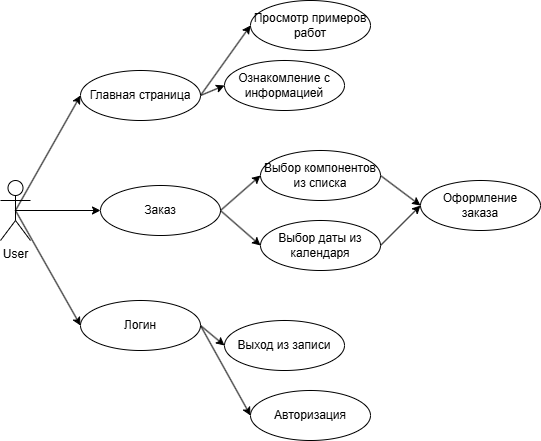
\includegraphics[width=1\linewidth]{userdp}
	\caption{Диаграмма прецедентов}
	\label{userdp:image}
\end{figure}
\clearpage
\begin{figure}[h]
	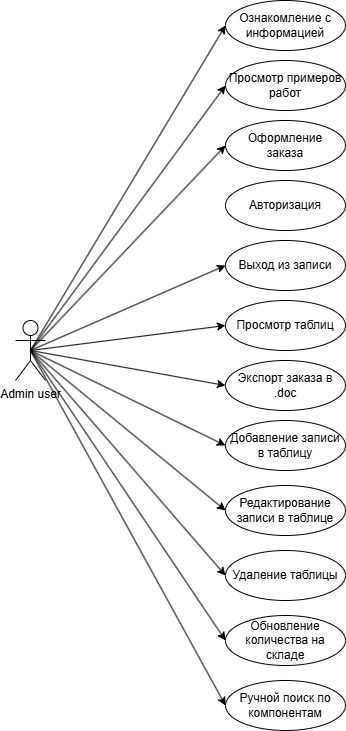
\includegraphics[width=1\linewidth]{aduserdp}
	\caption{Диаграмма прецедентов админа}
	\label{aduserdp:image}
\end{figure}
\clearpage

\subsubsection{Вариант использования «Ознакомление с информацией»}
Заинтересованные лица и их требования: пользователь желает узнать базовую информацию о Pc-Club, посмотреть на готовые сборки.
Предусловие: Открыт поисковик.
Постусловие: Пользователь заинтересован оформлением заказа у Pc-Club.
\begin{enumerate}
	\item Пользователь вводит адрес сайта/ищет его по названию Pc-Club.
	\item Пользователь попадает на главную страницу сервиса.
	\item Пользователь ознакамливается с преимуществами.
	\item Пользователь смотрит примеры выполненных работ.
\end{enumerate}

\subsubsection{Вариант использования «Оформление заказа»}
Заинтересованные лица и их требования: Заинтересованный пользователь хочет быстро и удобно оформить заказ.
Предусловие: Открыта главная страница сайта.
Постусловие: Был оформлен заказ и его запись отправилась в sql.
\begin{enumerate}
	\item Пользователь с помощью навигационной панели или кнопки "Начать сборку" 
	\item Пользователь попадает на страницу оформления заказа.
	\item Пользователь вводит данные.
	\item Пользователь выбирает даты из календаря.
	\item Пользователь нажимает на компонент.
	\item Пользователь вводит название интересующего компонента/выбирает из представленного.
	\item Пользователь нажимает на кнопку "оформить заказ".
	\item Система проверяет введенные данные через validator.
	\item Система вычитает из имеющегося числа компонентов, задействованные.
	\item Система отправляет подготовленный sql запрос с предоставленными данными.
	\item Запись добавляется в sql и заказ принят к работе.
\end{enumerate}

\subsubsection{Вариант использования «Регистрация»}
Заинтересованные лица и их требования: Пользователь хочет зарегистрировать новую учетную запись.
Предусловие: Открыта главная страница сайта.
Постусловие: Новая учетная запись сохранена в sql.
\begin{enumerate}
	\item Пользователь нажимает на кнопку "Войти" 
	\item Пользователь вводит логин в поле.
	\item Пользователь вводит пароль в поле.
	\item Пользователь нажимает зарегистрироваться.
	\item Система подготовленным sql запросом отправляет логин, хэш пароля в базу данных.
	\item Система сохраняет данные в sql и к ним можно обратиться.
\end{enumerate}

\subsubsection{Вариант использования «Вход(в админ)»}
Заинтересованные лица и их требования: Пользователь хочет войти под учетной записью администратора.
Предусловие: Открыта главная страница сайта.
Постусловие: Совершен вход в учетную запись администратора.
\begin{enumerate}
	\item Пользователь нажимает на кнопку "Войти" в навигации.
	\item Пользователь вводит логин администратора в поле.
	\item Пользователь вводит пароль администратора в поле.
	\item Пользователь нажимает войти.
	\item Система сравнивает логин и хэши паролей с имеющимися в sql.
	\item Система создает сессию, в нашем случае с правами администратора.
\end{enumerate}

\subsubsection{Вариант использования «Выход»}
Заинтересованные лица и их требования: Пользователь выйти из учетной записи.
Предусловие: Открыта главная страница сайта, пользователь авторизован.
Постусловие: Пользователь выходит из учетной записи.
\begin{enumerate}
	\item Пользователь нажимает на кнопку "Выход" в навигации.
	\item Система убирает все данные авторизации из сессии.
\end{enumerate}

\subsubsection{Вариант использования «Просмотр таблиц»}
Заинтересованные лица и их требования: Пользователь хочет посмотреть содержимое таблиц.
Предусловие: Открыта главная страница сайта, в текущей сессии есть права администратора.
Постусловие: Пользователь просматривает содержимое таблиц.
\begin{enumerate}
	\item Пользователь нажимает на кнопку "Админ панель" в навигации.
	\item Открывается страница панели администратора.
	\item Пользователь выбирает интересующий тип компонента.
	\item Система подгружает из sql интересующую таблицу.
	\item Система выводит интересующую таблицу.
	\item Пользователь просматривает содержимое таблицы.
\end{enumerate}

\subsubsection{Вариант использования «Редактирование таблиц»}
Заинтересованные лица и их требования: Пользователь хочет изменить запись в таблице.
Предусловие: Открыта админ панель.
Постусловие: Пользователь редактирует запись в таблице.
\begin{enumerate}
	\item Пользователь выбирает интересующую таблицу.
	\item Система подгружает из sql интересующую таблицу.
	\item Система выводит таблицу.
	\item Пользователь нажимает на кнопку "карандаш" у нужного элемента.
	\item Открывается страница для редактирования данных с имеющимися данными элемента.
	\item Пользователь меняет требуемые данные в формах и нажимает "Сохранить".
	\item Система проверяет введенные данные через validator.
	\item Система отправляет подготовленный sql запрос и обновляет данные в sql.
\end{enumerate}

\subsubsection{Вариант использования «Добавление в таблицу»}
Заинтересованные лица и их требования: Пользователь хочет добавить новую запись в таблицу.
Предусловие: Открыта админ панель.
Постусловие: Пользователь добавляет запись в таблицу.
\begin{enumerate}
	\item Пользователь выбирает интересующую таблицу.
	\item Система подгружает из sql интересующую таблицу.
	\item Система выводит таблицу.
	\item Пользователь нажимает на кнопку "+добавить" у нужной таблицы.
	\item Открывается страница для добавления нового элемента.
	\item Пользователь меняет требуемые данные в формах и нажимает "Добавить".
	\item Система проверяет введенные данные через validator.
	\item Система отправляет подготовленный sql запрос и сохраняет данные в sql.
\end{enumerate}

\subsubsection{Вариант использования «Удаление в таблице»}
Заинтересованные лица и их требования: Пользователь хочет удалить запись из таблицы.
Предусловие: Открыта админ панель.
Постусловие: Пользователь удаляет запись в таблице.
\begin{enumerate}
	\item Пользователь выбирает интересующую таблицу.
	\item Система подгружает из sql интересующую таблицу.
	\item Система выводит таблицу.
	\item Пользователь нажимает на кнопку с мусорным ведром у элемента.
	\item Браузер просит подтверждение действия.
	\item Пользователь нажимает "подтвердить".
	\item Система удаляет запись об элементе из sql.
\end{enumerate}

\subsubsection{Вариант использования «Обновления количества компонентов на складе»}
Заинтересованные лица и их требования: Пользователь хочет удалить запись из таблицы.
Предусловие: Открыта админ панель.
Постусловие: Пользователь обновляет количество компонента на складе.
\begin{enumerate}
	\item Пользователь нажимает на кнопку "склад" в навигации.
	\item Пользователь выбирает интересующую таблицу.
	\item Система подгружает из sql интересующую таблицу.
	\item Система выводит таблицу.
	\item Пользователь вводит новое количество компонента и нажимает "обновить".
	\item Система отправляет запрос в sql и сохраняет новое значение.
\end{enumerate}

%-------------------------------------------------------------------------------
\subsection{Требования пользователя к интерфейсу веб-приложения}

Композиция шаблона сайта представлена на рисунке ~\ref{indext:image}.

\begin{figure}[ht]

\includegraphics[width=1\linewidth]{indext}
\caption{Композиция шаблона сайта}
\label{indext:image}
\end{figure}
%\vspace{-\figureaboveskip} % двойной отступ не нужен (можно использовать, если раздел заканчивается картинкой)

\subsubsection{Гланая страница index}

Главная страница позволяет пользователю узнать основную информацию о деятельности сервис центра, посмотреть на существующие работы и должна заинтересовать его в заказе конкретно у Pc--Club. Главная страница, должна иметь элементы навигации для перемещения по сайту и получения доступа к разному контенту, аналогично и на других страницах.

\subsubsection{Страница авторизации login}

На странице авторизации пользователь или сотрудник могут совершить вход в существующую учетную запись или создать новую. Важно, регистрировать учетную запись администратора запрещено, можно только редактировать через систему. На странице должны быть аналогично index панель навигации и все необходимые инструменты для авторизации.

\subsubsection{Страница заказы orderform}

На этой странице пользователь или сотрудник может оформить заказ в удобном интерфейсе, после оформления заказа тот отправляется в базу данных на хранение. Каждый компонент можно удобно выбрать из выпадающего списка с поиском, а даты выбирать в открывающемся календаре.

\subsubsection{Страница админ панели editcontent}

Доступ к этой странице может получить только пользователь с учетной записью администратора, здесь можно редактировать какие вообще компоненты доступны, добавлять новые или удалять, просматривать информацию о заказах и редактировать её. Здесь у нас расширенная панель навигации позволяющая открыть к прочим еще страницу "склад", о ней дальше.

\subsubsection{Страница админ панели stockmanagment}

Доступ к этой странице аналогично, только у администратора, тут также расширенная панель навигации с доступом ко всем вкладкам. На самой странице сотрудник может пополнить количество любого недостающего компонента.

\subsection{Нефункциональные требования к программной системе}

\subsubsection{Требования к безопасности}
Для безопасности хранимых данных пользователей требуется сохранять пароли в формате  хэш-кодов. Стабильность работы самой базы данных может кто-то попытаться нарушить с помощью sql-иньекции, защититься от этого можно используя подготовленные sql запросы и валидацию принимаемых данных с помощью регулярных выражений.
\subsubsection{Требования к программному обеспечению}
Для реализации проекта потребуются такие Яп. как:
\begin{itemize}
	\item Html - разметка и структура сайта.
	\item Php - сценарии и взаимодействия.
	\item JavaScript - сложные функции и некоторая логика.	
	\item CSS - внешний вид страниц и кастомизация элементов.		
\end{itemize}

Также для создания базы данных и работы с ней на этапе разработки используется xampp, включающий в себя MySql для базы данных и Apache для создания локального веб-сервера. 

Для работы на персональном компьютере потребуется:
\begin{itemize}
	\item Операционная система: Windows (XP и выше), Mac OS X 10.4+, Linux.
	\item Оперативная память: минимум 1 ГБ.
	\item Веб-браузер: современные версии Chrome, Firefox, Edge и др.,поддерживающие EcmaScript 6.	
	\item Подключение к интернету: обязательно для работы с веб-приложениями.		
\end{itemize}

В свою очередь требования для удаленного сервера:
\begin{itemize}
	\item ОС Linux (Ubuntu, CentOS, Debian) или Windows Server, Linux предпочтительнее.
	\item Минимум 2–4 ГБ оперативной памяти.
	\item Процессор 1.5 GHz и выше.
	\item Объём дискового пространства от 10 ГБ и больше.
	\item Стабильный, высокоскоростной интернет с публичным IP-адресом.		
\end{itemize}
\subsection{Требования к оформлению документации}

Разработка программной документации и программного изделия должна производиться согласно ГОСТ 19.102-77 и ГОСТ 34.601-90. Единая система программной документации.
	\section{Технический проект}
\subsection{Общая характеристика организации решения задачи}

Необходимо разработать веб-приложение, которое организует работу в сервис-центре и поможет с его продвижением. Веб-приложение должно поспособствовать в организации работы сервиса Pc-Club и привлечь новых клиентов. Программно-информационная система представляет собой веб-приложение с архитектурой "клиент-сервер"

\subsection{Обоснование выбора средств разработки}
\subsubsection{Описание используемых технологий и языков программирования}

В процессе разработки веб-приложения потребовались языки для реализации разметки на странице, логики страницы, для настройки внешнего вида, также требуется создать базу данных для хранения всей информации. 

\paragraph{Язык разметки html}

В современном мире html является незаменимым инструментом при разработке любых веб-сайтов ведь позволяет достаточно удобно и структурировано располагать элементы на странице, добавлять таблицы и некоторое другое наполнение. Обычно на странице есть разделение на head, body, где в первом хранятся метаданные страницы, описание, ключевые слова итп., а во втором видимое содержимое страницы.

\paragraph{Язык программирования PHP}

PHP популярный серверный язык программирования, был разработан специально для веб-разработки, он встраивается в html. Главное отличие PHP от Js в том, что он исполняется на стороне сервера. Сам по себе получил широкое применение в создании серверной логики веб-сайтов/приложений, используется для взаимодействия с базами данных, обработки ввода пользователя и создания динамического контента.

\paragraph{Язык программирования JavaScript}

Js или же JavaScript ключевой язык программирования в современном frontend и важный инструмент в веб-разработке. Код выполняется в браузере и манипулирует DOM-деревом страницы, без нужды её перезагружать, позволяет отслеживать нажатия клавиш или клики мышкой в реальном времени.

\paragraph{Язык программирования CSS}

Это формальный язык описания внешнего вида страницы, определяющий стиль и расположение элементов на веб-странице. С помощью него можно тонко настраивать внешний вид элементов на странице, их расположение относительно друг друга. Когда страница создается браузер парсит html в DOM-дерево, а css в CSSOM-дерево, а после рендерит в общее дерево и отрисовывает готовую страницу.

\paragraph{База данных и Xampp}

Кросплатформенный  дистрибутив для сборки локального веб-сервера, содержит в себе Apache, MySQL нужные для реализации базы данных в разработке. Управление базой данных происходит через PhpMyAdmin - веб-приложение для администрирования БД, с помощью удобного графического интерфейса можно создавать, редактировать, а также установить на сервер. Взаимодействие с SQL происходит посредством специальных SQL запросов.

\subsection{Диаграмма компонентов и схема обмена данными между файлами компонента}

На рисунке \ref{thatsmedio1:image} изображена диаграмма компонентов для проектируемой системы. В диаграмме изображено отношение между компонентами и их взаимодействие.

\begin{figure}[ht]
\center{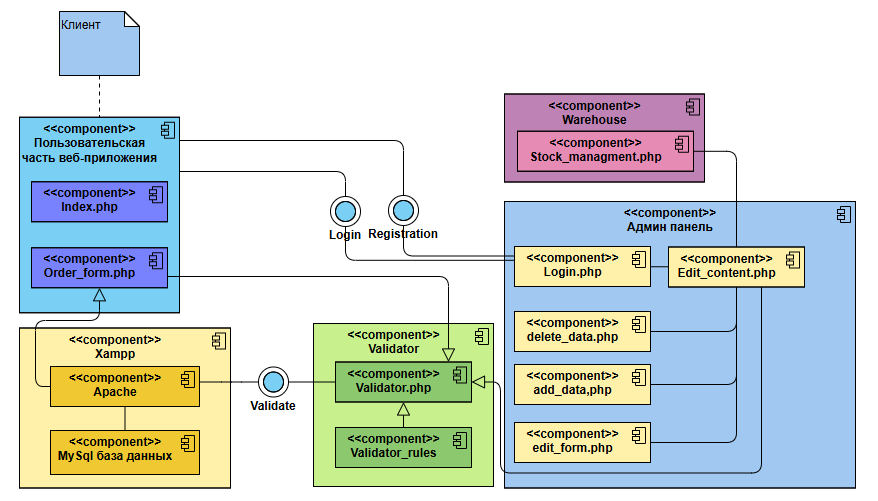
\includegraphics[width=1\linewidth]{thatsmedio1}}
\caption{Диаграмма компонентов}
\label{thatsmedio1:image}
\end{figure}

Любой компонент должен быть вызван в сценарии страницы web-сайта. Web-страница передает данные компоненту в момент вызова последнего.

Клиент взаимодействует с веб-сервером Apache который обрабатывает все php сценарии. Первой в очереди идет страница индекса, с нее можно попасть в orderform которая после проверки данных с помощью валидатора отправляет их в sql. Через index можно попасть в login где, происходит авторизация пользователя и если тот админ, то может попасть в панель. Панель позволяет редактировать, удалять, добавлять записи в sql, а так-же просматривать её содержимое. В случае редактирования/добавления проверяется через валидатор, перед отправкой в sql, для поддержания стабильности работы веб-приложения. В склад можно попасть с панели и редактировать количество имеющихся компонентов, получая и отправляя данные в sql.
\newpage

\subsubsection{Клиентская часть системы}
Роль: Интерфейс пользователя в браузере.
Содержит HTML/CSS-шаблоны.
JavaScript-логика (отправка запросов, валидация форм).
Отрисовка данных, полученных от сервера.

Отправляет AJAX/Fetch-запросы к API (PHP-скриптам).
Получает данные в формате JSON/HTML.
Выполняет первичную валидацию форм.

\subsubsection{Серверная часть системы}
Роль: Обработка бизнес-логики, работа с БД и генерация ответов для клиентской части.
Отображает контент (товары, заказы, формы).
Принимает данные от пользователя (регистрация, заказы, фильтры).
Обрабатывает http-запросы.
Взаимодействие с базой данных.
Формирует HTML/JSON-ответов.

\paragraph{Index.php} 
Роль: Главная страница приложения.
Точка входа приложения. Обрабатывает запросы к корневому URL.
Генерирует HTML главной страницы.
Содержит список популярных товаров или акций.

\paragraph{Order--form.php} 
Роль: Форма оформления заказа.
Выбор компонентов ПК и оформление заказа.
Валидирует введенные данные через Validator.php.
Сохраняет готовые заказы в БД.

\subsubsection{Серверная инфраструктура}
Для разработки использован стек XAMPP (Apache + MySQL + PHP). В промышленной среде приложение развертывается на:
\begin{enumerate}
	\item выделенном веб-сервере (Apache/Nginx);
	\item продьюшен-сервере MySQL/MariaDB;
	\item PHP с настроенным OPcache и ограничениями безопасности.
\end{enumerate}

\paragraph{MySQL база данных} 
Роль: Хранилище данных приложения.
Содержит таблицы: users, assembly, master и т.д.
Взаимодействует с PHP-скриптами через SQL-запросы (выборка, добавление, удаление данных).

\subsubsection{Login Registration}
Роль: Модуль аутентификации и регистрации.
Login.php: Проверяет логин/пароль, создает сессии.
Хэширует пароли.
Registration: Регистрирует новых пользователей, сохраняя данные в БД.

\subsubsection{Validator}
Роль: Проверка корректности данных.
Validator.php: Основной класс/скрипт валидации.
Validator--rules: Набор правил.
Используется в формах для предотвращения некорректных данных.

\subsubsection{Warehouse}
Роль: Управление складскими запасами.
Stock--management.php: Интерфейс для администраторов. Позволяет:
Просматривать остатки товаров.
Редактировать количество товаров.
Связан с таблицей stock в БД.

\subsubsection{Панель администратора}
Роль: Панель управления для администраторов.
Доступна после авторизации через Login.php.
Включает:
Редактирование и добавление товаров.
Просмотр заказов и отчетов.
Экспорт заказов в файл.

\paragraph{delete--data.php}
Роль: Удаление записей из БД.
Принимает ID записи (например, товара или пользователя).
Выполняет SQL-запрос DELETE (после проверки прав доступа).
\paragraph{add--data.php}
Роль: Добавление новых данных в БД.
Принимает данные из форм.
Выполняет SQL-запрос INSERT.
Взаимодействует с Validator.php для проверки входных данных.

\paragraph{edit--form.php}
Роль: Форма редактирования существующих данных.
Загружает текущие данные из БД.
Позволяет внести изменения.
Напрямую выполняет UPDATE.

\subsubsection{Взаимодействие модулей}
Пользователь открывает Index.php, переходит к Order--form.php.
Клиентская часть отправляет данные формы, серверный скрипт проверяет авторизацию, проверяет через Validator.php, если цена неотрицательное число, если дата оформления и доставки корректные, если все элементы не пустые и существуют, сохраняет заказ в БД.
Админ входит через Login.php, получает доступ к Админ панели.
В Админ панели:
Для удаления товара: delete--data.php.
Для редактирования: edit--form.php.
Для добавлени: add--data.php.

\newpage
\subsection{Структура базы данных sql и таблиц}

Реляционная схема (рис.~\ref{struct:image}) отражает отношение данных в sql в удобном табличном виде.

\vspace{-8mm} 
\begin{figure}[ht]
\center{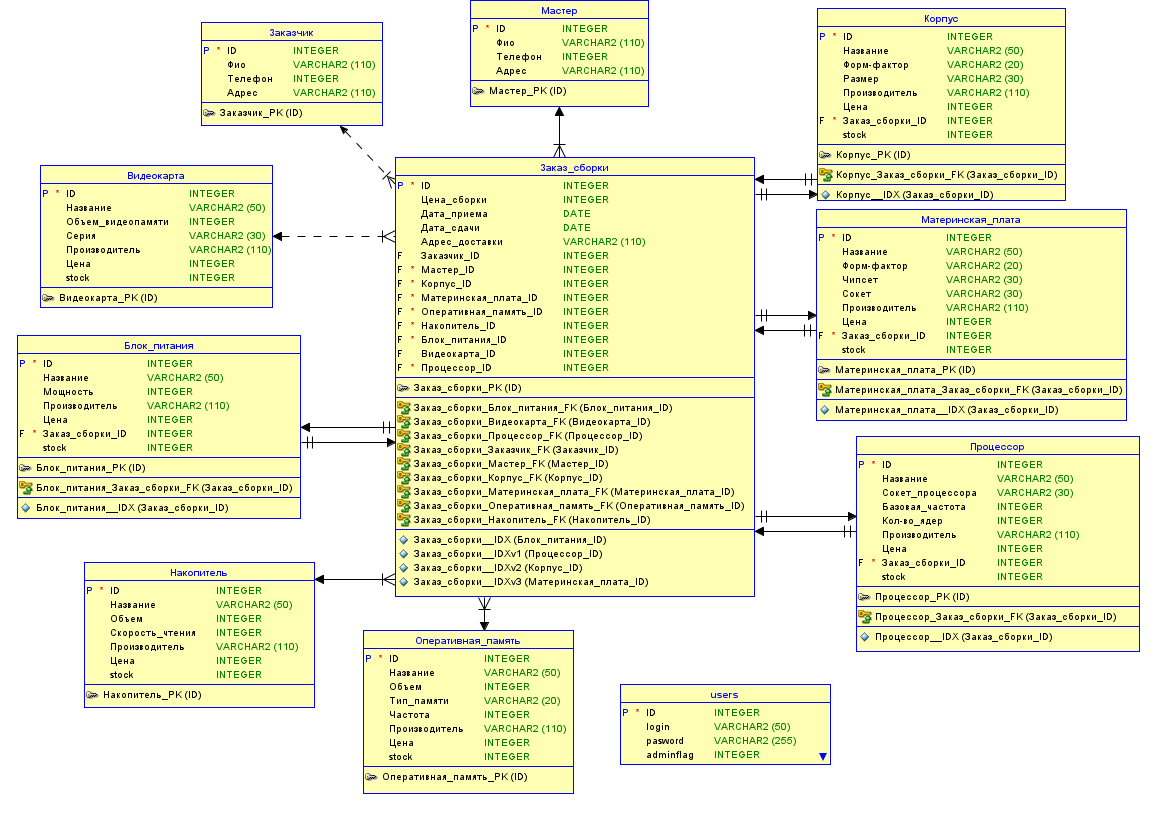
\includegraphics[width=1.00\linewidth]{struct}}
\caption{Реляционная схема базы данных}
\label{struct:image}
\end{figure}

Все таблицы сходятся к одной таблице assembly, которая представляет собой сам "заказ". Также есть отдельная таблица users, нужна она для хранения данных пользователей.
В таблицах 3.1-3.11 представлены описания структур таблиц базы данных:

\renewcommand{\arraystretch}{0.8}

% Таблица Customer
\begin{xltabular}{\textwidth}{|X|X|p{4.0cm}|X|X|}
	\caption{Описание таблицы Customer с кратким именем CTR\label{tab:customer}}\\
	\hline
	\multicolumn{1}{|c|}{Имя таблицы} & \multicolumn{4}{c|}{Краткое имя таблицы} \\ \hline
	\multicolumn{1}{|c|}{Customer} & \multicolumn{4}{c|}{CTR} \\ \hline
	\multicolumn{1}{|c|}{Key Type} & \multicolumn{1}{c|}{Optionality} & \multicolumn{1}{c|}{Column name} & \multicolumn{1}{c|}{Data type} & \multicolumn{1}{c|}{Size} \\ \hline
	pk & * & ctr\_id & NUMBER & 13 \\ \hline
	& * & full\_name & VARCHAR2 & 110 \\ \hline
	& * & phone\_namber & NUMBER & 11 \\ \hline
	& * & legal\_address & VARCHAR2 & 110 \\ \hline
\end{xltabular}

% Таблица Master
\begin{xltabular}{\textwidth}{|X|X|p{4.0cm}|X|X|}
	\caption{Описание таблицы Master с кратким именем MTR\label{tab:master}}\\
	\hline
	\multicolumn{1}{|c|}{Имя таблицы} & \multicolumn{4}{c|}{Краткое имя таблицы} \\ \hline
	\multicolumn{1}{|c|}{Master} & \multicolumn{4}{c|}{MTR} \\ \hline
	Key Type & Optionality & Column name & Data type & Size \\ \hline
	pk & * & mtr\_id & NUMBER & 13 \\ \hline
	& * & full\_name & VARCHAR2 & 110 \\ \hline
	& * & phone\_namber & NUMBER & 11 \\ \hline
	& * & legal\_address & VARCHAR2 & 110 \\ \hline
	& * & legal\_address & VARCHAR2 & 110 \\ \hline
\end{xltabular}

% Таблица Case
\begin{xltabular}{\textwidth}{|X|X|p{4.0cm}|X|X|}
	\caption{Описание таблицы Mcase с кратким именем CSE\label{tab:case}}\\
	\hline
	\multicolumn{1}{|c|}{Имя таблицы} & \multicolumn{4}{c|}{Краткое имя таблицы} \\ \hline
	\multicolumn{1}{|c|}{Mcase} & \multicolumn{4}{c|}{CSE} \\ \hline
	Key Type & Optionality & Column name & Data type & Size \\ \hline
	pk & * & cse\_id & NUMBER & 13 \\ \hline
	& * & case\_name & VARCHAR2 & 50 \\ \hline
	& * & form\_factor & VARCHAR2 & 20 \\ \hline
	& * & case\_size & VARCHAR2 & 30 \\ \hline
	& * & case\_manufacturer & VARCHAR2 & 110 \\ \hline
	& * & price & NUMBER & 30 \\ \hline
	& * & stock & NUMBER & 5 \\ \hline
\end{xltabular}

% Таблица Motherboard
\begin{xltabular}{\textwidth}{|X|X|p{4.0cm}|X|X|}
	\caption{Описание таблицы Motherboard с кратким именем MBD\label{tab:motherboard}}\\
	\hline
	\multicolumn{1}{|c|}{Имя таблицы} & \multicolumn{4}{c|}{Краткое имя таблицы} \\ \hline
	\multicolumn{1}{|c|}{Motherboard} & \multicolumn{4}{c|}{MBD} \\ \hline
	Key Type & Optionality & Column name & Data type & Size \\ \hline
	pk & * & mbd\_id & NUMBER & 13 \\ \hline
	& * & motherboard\_name & VARCHAR2 & 50 \\ \hline
	& * & form\_factor & VARCHAR2 & 20 \\ \hline
	& * & chipset & VARCHAR2 & 30 \\ \hline
	& * & socket & VARCHAR2 & 30 \\ \hline
	& * & board\_manufacturer & VARCHAR2 & 110 \\ \hline
	& * & price & NUMBER & 30 \\ \hline
	& * & stock & NUMBER & 5 \\ \hline
\end{xltabular}

% Таблица Processor
\begin{xltabular}{\textwidth}{|X|X|p{4.0cm}|X|X|}
	\caption{Описание таблицы Processor с кратким именем CPU\label{tab:processor}}\\
	\hline
	\multicolumn{1}{|c|}{Имя таблицы} & \multicolumn{4}{c|}{Краткое имя таблицы} \\ \hline
	\multicolumn{1}{|c|}{Processor} & \multicolumn{4}{c|}{CPU} \\ \hline
	Key Type & Optionality & Column name & Data type & Size \\ \hline
	pk & * & cpu\_id & NUMBER & 13 \\ \hline
	& * & unit\_name & VARCHAR2 & 50 \\ \hline
	& * & socket & VARCHAR2 & 30 \\ \hline
	& * & base\_frequency & NUMBER & 20 \\ \hline
	& * & number\_of\_cores & NUMBER & 10 \\ \hline
	& * & cpu\_manufacturer & VARCHAR2 & 110 \\ \hline
	& * & price & NUMBER & 30 \\ \hline
	& * & stock & NUMBER & 5 \\ \hline
\end{xltabular}

% Таблица RAM
\begin{xltabular}{\textwidth}{|X|X|p{4.0cm}|X|X|}
	\caption{Описание таблицы RAM с кратким именем RAM\label{tab:ram}}\\
	\hline
	\multicolumn{1}{|c|}{Имя таблицы} & \multicolumn{4}{c|}{Краткое имя таблицы} \\ \hline
	\multicolumn{1}{|c|}{RAM} & \multicolumn{4}{c|}{RAM} \\ \hline
	Key Type & Optionality & Column name & Data type & Size \\ \hline
	pk & * & ram\_id & NUMBER & 13 \\ \hline
	& * & ram\_name & VARCHAR2 & 50 \\ \hline
	& * & memory\_size & NUMBER & 30 \\ \hline
	& * & type & VARCHAR2 & 10 \\ \hline
	& * & base\_frequency & NUMBER & 20 \\ \hline
	& * & ram\_manufacturer & VARCHAR2 & 110 \\ \hline
	& * & price & NUMBER & 30 \\ \hline
	& * & stock & NUMBER & 5 \\ \hline
\end{xltabular}

% Таблица Storage
\begin{xltabular}{\textwidth}{|X|X|p{4.0cm}|X|X|}
	\caption{Описание таблицы Storage с кратким именем SDU\label{tab:storage}}\\
	\hline
	\multicolumn{1}{|c|}{Имя таблицы} & \multicolumn{4}{c|}{Краткое имя таблицы} \\ \hline
	\multicolumn{1}{|c|}{Storage} & \multicolumn{4}{c|}{SDU} \\ \hline
	Key Type & Optionality & Column name & Data type & Size \\ \hline
	pk & * & sdu\_id & NUMBER & 13 \\ \hline
	& * & storage\_name & VARCHAR2 & 50 \\ \hline
	& * & storage\_capacity & NUMBER & 20 \\ \hline
	& * & reading\_speed & NUMBER & 20 \\ \hline
	& * & sdu\_type & VARCHAR2 & 20 \\ \hline
	& * & sdu\_manufacturer & VARCHAR2 & 110 \\ \hline
	& * & price & NUMBER & 30 \\ \hline
	& * & stock & NUMBER & 5 \\ \hline
\end{xltabular}

% Таблица Power Unit
\begin{xltabular}{\textwidth}{|X|X|p{4.0cm}|X|X|}
	\caption{Описание таблицы Power\_unit с кратким именем PSU\label{tab:psu}}\\
	\hline
	\multicolumn{1}{|c|}{Имя таблицы} & \multicolumn{4}{c|}{Краткое имя таблицы} \\ \hline
	\multicolumn{1}{|c|}{Power\_unit} & \multicolumn{4}{c|}{PSU} \\ \hline
	Key Type & Optionality & Column name & Data type & Size \\ \hline
	pk & * & psu\_id & NUMBER & 13 \\ \hline
	& * & power\_name & VARCHAR2 & 50 \\ \hline
	& * & capability & NUMBER & 20 \\ \hline
	& * & power\_manufacturer & VARCHAR2 & 110 \\ \hline
	& * & price & NUMBER & 30 \\ \hline
	& * & stock & NUMBER & 5 \\ \hline
\end{xltabular}

% Таблица Graphics Card
\begin{xltabular}{\textwidth}{|X|X|p{4.0cm}|X|X|}
	\caption{Описание таблицы Graphics\_card с кратким именем GPU\label{tab:gpu}}\\
	\hline
	\multicolumn{1}{|c|}{Имя таблицы} & \multicolumn{4}{c|}{Краткое имя таблицы} \\ \hline
	\multicolumn{1}{|c|}{Graphics\_card} & \multicolumn{4}{c|}{GPU} \\ \hline
	Key Type & Optionality & Column name & Data type & Size \\ \hline
	pk & * & gpu\_id & NUMBER & 13 \\ \hline
	& * & gpu\_name & VARCHAR2 & 50 \\ \hline
	& * & gmemory\_size & NUMBER & 20 \\ \hline
	& * & gpu\_series & VARCHAR2 & 30 \\ \hline
	& * & gpu\_manufacturer & VARCHAR2 & 110 \\ \hline
	& * & price & NUMBER & 30 \\ \hline
	& * & stock & NUMBER & 5 \\ \hline
\end{xltabular}

% Таблица Assembly Order
\begin{xltabular}{\textwidth}{|X|X|p{4.0cm}|X|X|}
	\caption{Описание таблицы Assembly\_order с кратким именем ASO\label{tab:aso}}\\
	\hline
	\multicolumn{1}{|c|}{Имя таблицы} & \multicolumn{4}{c|}{Краткое имя таблицы} \\ \hline
	\multicolumn{1}{|c|}{Assembly\_order} & \multicolumn{4}{c|}{ASO} \\ \hline
	Key Type & Optionality & Column name & Data type & Size \\ \hline
	pk & * & assembly\_order\_id & NUMBER & 13 \\ \hline
	& * & assembly\_price & NUMBER & 50 \\ \hline
	& * & date\_of\_admission & DATE & 10 \\ \hline
	& * & date\_of\_delivery & DATE & 10 \\ \hline
	& * & delivery\_address & VARCHAR2 & 110 \\ \hline
	fk & * & ctr\_id & NUMBER & 13 \\ \hline
	fk & * & mtr\_id & NUMBER & 13 \\ \hline
	fk & * & case\_id & NUMBER & 13 \\ \hline
	fk & * & mbd\_id & NUMBER & 13 \\ \hline
	fk & * & cpu\_id & NUMBER & 13 \\ \hline
	fk & * & ram\_id & NUMBER & 13 \\ \hline
	fk & * & sdu\_id & NUMBER & 13 \\ \hline
	fk & * & psu\_id & NUMBER & 13 \\ \hline
	fk & * & gpu\_id & NUMBER & 13 \\ \hline
\end{xltabular}

% Таблица Users
\begin{xltabular}{\textwidth}{|X|X|p{4.0cm}|X|X|}
	\caption{Описание таблицы Users с кратким именем USR\label{tab:users}}\\
	\hline
	\multicolumn{1}{|c|}{Имя таблицы} & \multicolumn{4}{c|}{Краткое имя таблицы} \\ \hline
	\multicolumn{1}{|c|}{Users} & \multicolumn{4}{c|}{USR} \\ \hline
	Key Type & Optionality & Column name & Data type & Size \\ \hline
	pk & * & id & NUMBER & 11 \\ \hline
	& * & login & VARCHAR & 50 \\ \hline
	& * & password & VARCHAR & 255 \\ \hline
	& * & adminflag & NUMBER & 1 \\ \hline
\end{xltabular}

\renewcommand{\arraystretch}{1.0}



	\ifПрактика{}\else{
		\section{Рабочий проект}
\subsection{Спецификация компонентов и классов системы}
\subsubsection{Спецификация пользовательской части системы}
Главная страница системы
Предоставляет точку входа в приложение, отображает маркетинговую информацию, преимущества компании и примеры работ. Служит навигационным хабом для перехода к ключевым функциям системы.

Взаимодействия:
\begin{itemize}
	\item Связь с order\_form.php;
	\item интеграция с edit\_content.php для административного доступа;
	\item использование logout.php для смены учетной записи.
\end{itemize}

Использует CSS Grid и медиазапросы для перестроения макета на мобильных устройствах.
Горизонтальная карусель с hover-эффектами на изображениях.

Зависимости:
\begin{itemize}
\item внешний CSS-файл: style.css;
\item локальные изображения: images/pc\_build1-5.jpg;
\item поддержка PHP для обработки даты.
\end{itemize}

Спецификация компонента: order\_form.php
Система оформления заказов
Обрабатывает создание заказов на сборку компьютеров. Управляет выбором компонентов, валидацией данных и транзакционным обновлением остатков на складе. 

Взаимодействия:
\begin{itemize}
	\item интеграция с MySQL БД;
	\item связь с index.php и edit\_content.php через навигацию;
	\item использование logout.php для смены пользователя.
\end{itemize}

Безопасность и валидация:
Осуществляется через подготовленные SQL-запросы (prepare + bind\_param), экранирование вывода (htmlspecialchars).

Валидация ввода: 
Проверяется формат цены, должна быть числом и ограничение по размеру, контролирует даты, предотвращает ввод некорректного формата данных с помощью выпадающего календаря и проверяет даты на корректный ввод, каждый компонент предлагается из SQL, проверяется его наличие и существование. В таблице ~\ref{class:table} показаны основные функции компонента.
\renewcommand{\arraystretch}{0.8}
\begin{xltabular}{\textwidth}{|p{4.0cm}|>{\setlength{\baselineskip}{0.7\baselineskip}}p{5.5cm}|>{\setlength{\baselineskip}{0.7\baselineskip}}X|}
	\caption{Описание функций и скриптов, используемых в приложении\label{class:table}}\\
	\hline \centrow Название компонента & \centrow Описание & \centrow Методы / Действия \\
	\hline \endfirsthead
	\caption*{Продолжение таблицы \ref{class:table}}\\
	\hline \centrow Название компонента & \centrow Описание & \centrow Методы / Действия \\
	\hline \endhead
	
	getComponents & Получает массив данных из таблицы БД (комплектующие, клиенты, мастера) & Формирует и выполняет SELECT-запрос, возвращает ассоциативный массив \\\hline
	
	get\_id\_column & Возвращает имя id-столбца для таблицы комплектующих & Сопоставляет название таблицы с её id-столбцом \\\hline
	
	get\_table\_name & Возвращает имя таблицы по имени id-поля & Сопоставляет поле с таблицей, возвращает строку \\\hline
	
	toggleDropdown & Переключает видимость выпадающего списка (dropdown) & Находит список по id, переключает класс show, фокусирует input \\\hline
	
	showDropdown & Показывает нужный выпадающий список & Скрывает все списки, затем показывает нужный (добавляет класс show) \\\hline
	
	filterDropdown & Фильтрует элементы списка по введённому тексту & Сравнивает текст каждого li с введённым значением, скрывает/показывает элементы \\\hline
	
\end{xltabular}
\renewcommand{\arraystretch}{1.0}

\subsubsection{Спецификация панели администратора}
Основная страница (edit\_content.php)
Центральный интерфейс управления данными системы. Предоставляет CRUD-операции для всех сущностей: сборки, мастера, клиенты, комплектующие. Реализует поиск, фильтрацию и экспорт данных. В таблице ~\ref{admin:table} показаны основные функции компонента.

Взаимодействия:
\begin{itemize}
	\item интеграция с MySQL БД через параметризованные запросы;
	\item связь с add\_data.php для создания записей;
	\item интеграция с edit\_form.php для редактирования;
	\item использование delete\_data.php для удаления;
	\item экспорт в DOC через export.php.
\end{itemize}

Безопасность:
\begin{itemize}
	\item проверка сессии и флага администратора (adminflag=1);
	\item экранирование вывода (htmlspecialchars);
	\item подготовленные SQL-запросы.
\end{itemize}

Особенности:
\begin{itemize}
	\item адаптивный дизайн с медиазапросами;
	\item динамическая загрузка таблиц по выбранной категории;
	\item интерактивные элементы управления.
\end{itemize}

Добавление и редактирование записи (add\_data.php и edit\_form.php)
Два довольно схожих интерфейса, предназначение которых взаимодействие с записями, добавление и редактирование существующих. 

Взаимодействия:
\begin{itemize}
	\item валидация через validator.php;
	\item интеграция с edit\_content.php для редиректа;
	\item использование сессий для сохранения состояния.
\end{itemize}

Валидация:
\begin{itemize}
	\item применение правил из validation\_rules.php;
	\item обработка ошибок через сессии;
	\item автоматическое определение ID-колонок.
\end{itemize}

Безопасность:
\begin{itemize}
	\item проверка прав администратора;
	\item параметризованные SQL-запросы;
	\item экранирование вывода.
\end{itemize}

Особенности:
\begin{itemize}
	\item автозаполнение полей текущими значениями
	\item динамическое построение формы;
	\item отображение ошибок валидации;
	\item универсальный дизайн для всех таблиц;
	\item сохранение введенных данных при ошибках.
\end{itemize}

Удаление (delete\_data.php)
Скрипт обработки удаления записей из БД. Вызывается асинхронно через AJAX.

Взаимодействия:
\begin{itemize}
	\item принимает POST-запросы от edit\_content.php;
	\item интеграция с MySQL через подготовленные запросы.
\end{itemize}

Безопасность:
\begin{itemize}
	\item автоматическое определение первичных ключей;
	\item подтверждение операции через JavaScript;
	\item отсутствие прямого доступа (только POST).
\end{itemize}

Особенности:
\begin{itemize}
	\item универсальная работа для всех таблиц;
	\item возврат текстовых статусов операции.
\end{itemize}

Авторизация (login.php)
Система аутентификации пользователей с разделением прав (администратор/клиент).

Взаимодействия:
\begin{itemize}
	\item интеграция с БД для проверки учетных данных;
	\item редирект на edit\_content.php (админ) или index.php (клиент);
	\item связь с сессиями PHP.
\end{itemize}

Безопасность:
\begin{itemize}
	\item хеширование паролей (password\_hash/verify);
	\item подготовленные SQL-запросы.
\end{itemize}

Особенности:
\begin{itemize}
	\item комбинированная форма входа/регистрации;
	\item визуальная обратная связь при ошибках.
\end{itemize}

\renewcommand{\arraystretch}{0.8}
\begin{xltabular}{\textwidth}{|p{4.0cm}|>{\setlength{\baselineskip}{0.7\baselineskip}}p{5.5cm}|>{\setlength{\baselineskip}{0.7\baselineskip}}X|}
	\caption{Описание функций и скриптов админ-панели\label{admin:table}}\\
	\hline \centrow Название компонента & \centrow Описание & \centrow Методы / Действия \\
	\hline \endfirsthead
	\caption*{Продолжение таблицы \ref{admin:table}}\\
	\hline \centrow Название компонента & \centrow Описание & \centrow Методы / Действия \\
	\hline \endhead
	
	getIdColumn() & Определяет имя первичного ключа для таблицы & Анализирует название таблицы, возвращает имя ID-колонки \\ \hline
	
	editData() & Редактирование записи & Перенаправляет на edit\_form.php с параметрами таблицы и ID \\ \hline
	
	deleteData() & Удаление записи & Отправляет AJAX-запрос в delete\_data.php, обновляет интерфейс \\ \hline
	
	exportAssembly() & Экспорт данных сборки & Открывает export.php в новом окне для генерации DOC-файла \\ \hline
	
	validate() & Проверка данных формы & Применяет правила из validation\_rules.php, возвращает ошибки \\ \hline
	
	searchDropdown() & Фильтрация данных в таблице & Формирует SQL-запрос с LIKE, динамически обновляет таблицу \\ \hline
	
	toggleDropdown() & Управление элементами UI & Переключает видимость выпадающих списков, управляет CSS-классами \\ \hline
	
\end{xltabular}
\renewcommand{\arraystretch}{1.0}

\subsubsection{Спецификация модуля валидации}
Универсальный механизм валидации данных для всех сущностей системы. Обеспечивает целостность данных при операциях CRUD.

Инициализация:
\begin{itemize}
	\item принимает подключение к БД (mysqli) и правила валидации;
	\item сохраняет контекст для проверок.
\end{itemize}

Метод validate():
\begin{itemize}
	\item основной интерфейс проверки данных;
	\item проверка обязательности поля;
	\item валидация типа данных;
	\item проверка длины;		
	\item соответствие regex-паттерну;
	\item верификация внешних ключей.
\end{itemize}

Особенности:
\begin{itemize}
	\item гибкая система сообщений об ошибках;
	\item каскадная проверка (остановка после первой ошибки поля);
	\item поддержка пользовательских сообщений;
	\item интеграция с БД для проверки внешних ключей.
\end{itemize}

Правила валидации (validation\_rules.php)
Гибкий список содержащий все правила валидации для validator.php, структура правил представлена на рисунке ~\ref{fig:strcode1}. В таблице ~\ref{valid} представлены методы класса validator.

\begin{figure}[ht]
	\begin{lstlisting}[language=Php]
			[
			'table_name' => [
			'field_name' => [
			'rule_type' => rule_value,
			'messages' => [
			'error_type' => 'Текст ошибки']]]
			]
			\end{lstlisting}
			\caption{Структура правил валидации}
			\label{fig:strcode1}
		\end{figure}

\renewcommand{\arraystretch}{0.8}
\begin{xltabular}{\textwidth}{|p{4.0cm}|p{5.5cm}|X|}
	\caption{Методы класса \texttt{validator} \label{valid}}\\
	\hline \centrow Название метода & \centrow Описание & \centrow Ключевые действия \\
	\hline \endfirsthead
	\caption*{Продолжение таблицы \ref{valid}}\\
	\hline \centrow Название метода & \centrow Описание & \centrow Ключевые действия \\
	\hline \endhead
	
	\texttt{\_\_construct()} & Конструктор класса, инициализирует соединение с БД и правила валидации & Сохраняет ссылку на объект mysqli и массив правил \\\hline
	
	\texttt{validate()} & Проверяет массив данных по правилам для указанной таблицы & Обходит все поля и применяет: required, type, max, pattern, foreign; возвращает массив ошибок \\\hline
	
	\texttt{validateType()} & Проверяет тип значения (число, дата) & Проверяет is\_numeric или формат даты, добавляет ошибку при несоответствии \\\hline
	
	\texttt{validateMaxLength()} & Проверяет максимальную длину значения & Сравнивает длину строки с лимитом, добавляет ошибку если превышено \\\hline
	
	\texttt{validatePattern()} & Проверяет соответствие значения регулярному выражению & Выполняет preg\_match по заданному паттерну, добавляет ошибку если не совпадает \\\hline
	
	\texttt{validateForeign()} & Проверяет существование значения во внешней таблице (foreign key) & Делит строку на имя таблицы и столбца, вызывает existsInTable \\\hline
	
	\texttt{addError()} & Добавляет ошибку для поля & Записывает сообщение об ошибке в массив ошибок \\\hline
	
	\texttt{existsInTable()} & Проверяет наличие значения в указанной таблице и столбце & Выполняет SELECT COUNT(*) с параметром, возвращает true/false \\\hline
	
\end{xltabular}
\renewcommand{\arraystretch}{1.0}

\subsubsection{Спецификация модуля склада}
Предоставляет администратору интерфейс для управления запасами комплектующих. Позволяет просматривать и обновлять количество товаров в категориях с фильтрацией и поиском. В таблице ~\ref{stock} представленные основные методы страницы склада.

Взаимодействия:
\begin{itemize}
	\item интеграция с MySQL БД для получения/обновления данных;
	\item ссылки на остальные страницы системы;
	\item использование logout.php для смены пользователя.
\end{itemize}

Безопасность и валидация:
\begin{itemize}
	\item проверка прав администратора;
	\item подготовленные SQL-запросы;
	\item экранирование вывода.
	\item Ограничение ввода (положительные числа).
\end{itemize}

\renewcommand{\arraystretch}{0.8}
\begin{xltabular}{\textwidth}{|p{4cm}|p{5.5cm}|X|}
	\caption{Ключевые методы склада \label{stock}}\\
	\hline \centrow Название компонента & \centrow Описание & \centrow Ключевые действия \\
	\hline \endfirsthead
	\caption*{Продолжение таблицы \ref{stock}}\\
	\hline \centrow Название метода & \centrow Описание & \centrow Ключевые действия \\
	\hline \endhead
	
	\texttt{if (\$\_SERVER['REQUEST\_ METHOD'] == 'POST' \&\& isset(\$\_POST['update\_ stock']))} & Обработка обновления остатков & Получает данные из POST, выполняет UPDATE через prepared statement, выставляет сообщения в \_SESSION \\ \hline
	
	\texttt{select name="table"} & Выбор категории комплектующих & Меняет таблицу для отображения/редактирования остатков, отправляет форму при изменении \\ \hline
	
	\texttt{input name="search"} & Поиск по названию комплектующих & Передаёт поисковый запрос через GET, используется в SQL-LIKE \\ \hline
	
	\texttt{match(\$selected \_table)\{\}} & Определение имени столбца названия & Выбирает нужный столбец (gpu\_name, ram\_name и т.д.) для SQL-запроса \\ \hline
\end{xltabular}
\renewcommand{\arraystretch}{1.0}

\subsubsection{Взаимодействие компонентов системы}
Пользователь переходит с index.php на order\_form.php, где заполняет данные заказа. При отправке формы order\_form.php обращается к validator.php для проверки: авторизации пользователя, неотрицательной цены, корректности дат и наличия комплектующих в базе данных. После успешной валидации данные сохраняются в базе, при этом автоматически обновляются остатки.

Администратор авторизуется через login.php с проверкой флага adminflag=1, получая доступ к edit\_content.php, который является панелью для административных операций. Отсюда доступны функции удаления данных через delete\_data.php, редактирования через edit\_form.php (загрузка текущих данных, валидация, сохранение) и добавления через add\_data.php (пустая форма, валидация, запись в базу).

validator.php обслуживает все критические операции: проверку данных при заказах, редактировании и добавлении, stock\_management.php позволяет отслеживать и редактировать количество компонентов на складе. Все компоненты взаимодействуют с базой данных посредством параметризованных запросов для обеспечения безопасности и надежности.


\subsection{Описание элементов интерфейса пользователя}

На рисунке \ref{index:image} главная страница сайта PC-Club содержит информацию, навигацию, пример работ.

\begin{enumerate}
	\item Панель навигации.
	\item Переход на страницу админ панели.
	\item Переход на страницу оформления.
	\item Смена учетной записи.
	\item Информационный блок.
	\item Переход к оформлению.
	\item Информационный блок, преимущества PC-Club.
	\item Блок с примерами работ.
	\item Кастомный скролл.
	\item Footer сайта с информацией.
\end{enumerate}

\begin{figure}[ht]
\center{
\includegraphics[width=1\linewidth]{index}}
\caption{Главная страница сайта.}
\label{index:image}
\end{figure}

\newpage 
На рисунке \ref{main:image} представлено меню оформления заказа,  в каждом поле можно вписать вручную или выбрать из выпадающего списка.
\begin{enumerate}
	\item Переход на страницу админ панели.
	\item Переход на главную страницу.
	\item Смена учетной записи.
	\item Простая форма ввода только чисел для цены.
	\item Форма ввода с календарем для вывода дат, проверяет на корректность.
	\item Простая форма ввода для адреса.
	\item Выбор из выпадающего списка.
	\item Выбор из выпадающего списка с возможностью ручного ввода.
	\item Кнопка собирает информацию с форм и отправляет в sql.
	\item Выпадающее меню.
	\item Поле ручного ввода/поиска по компонентам в sql.
	\item Кнопка развернуть.
	\item Виды комплектующих из sql.
	\item Сколько этих комплектующих осталось на складе.
\end{enumerate}

\begin{figure}[H]
\center{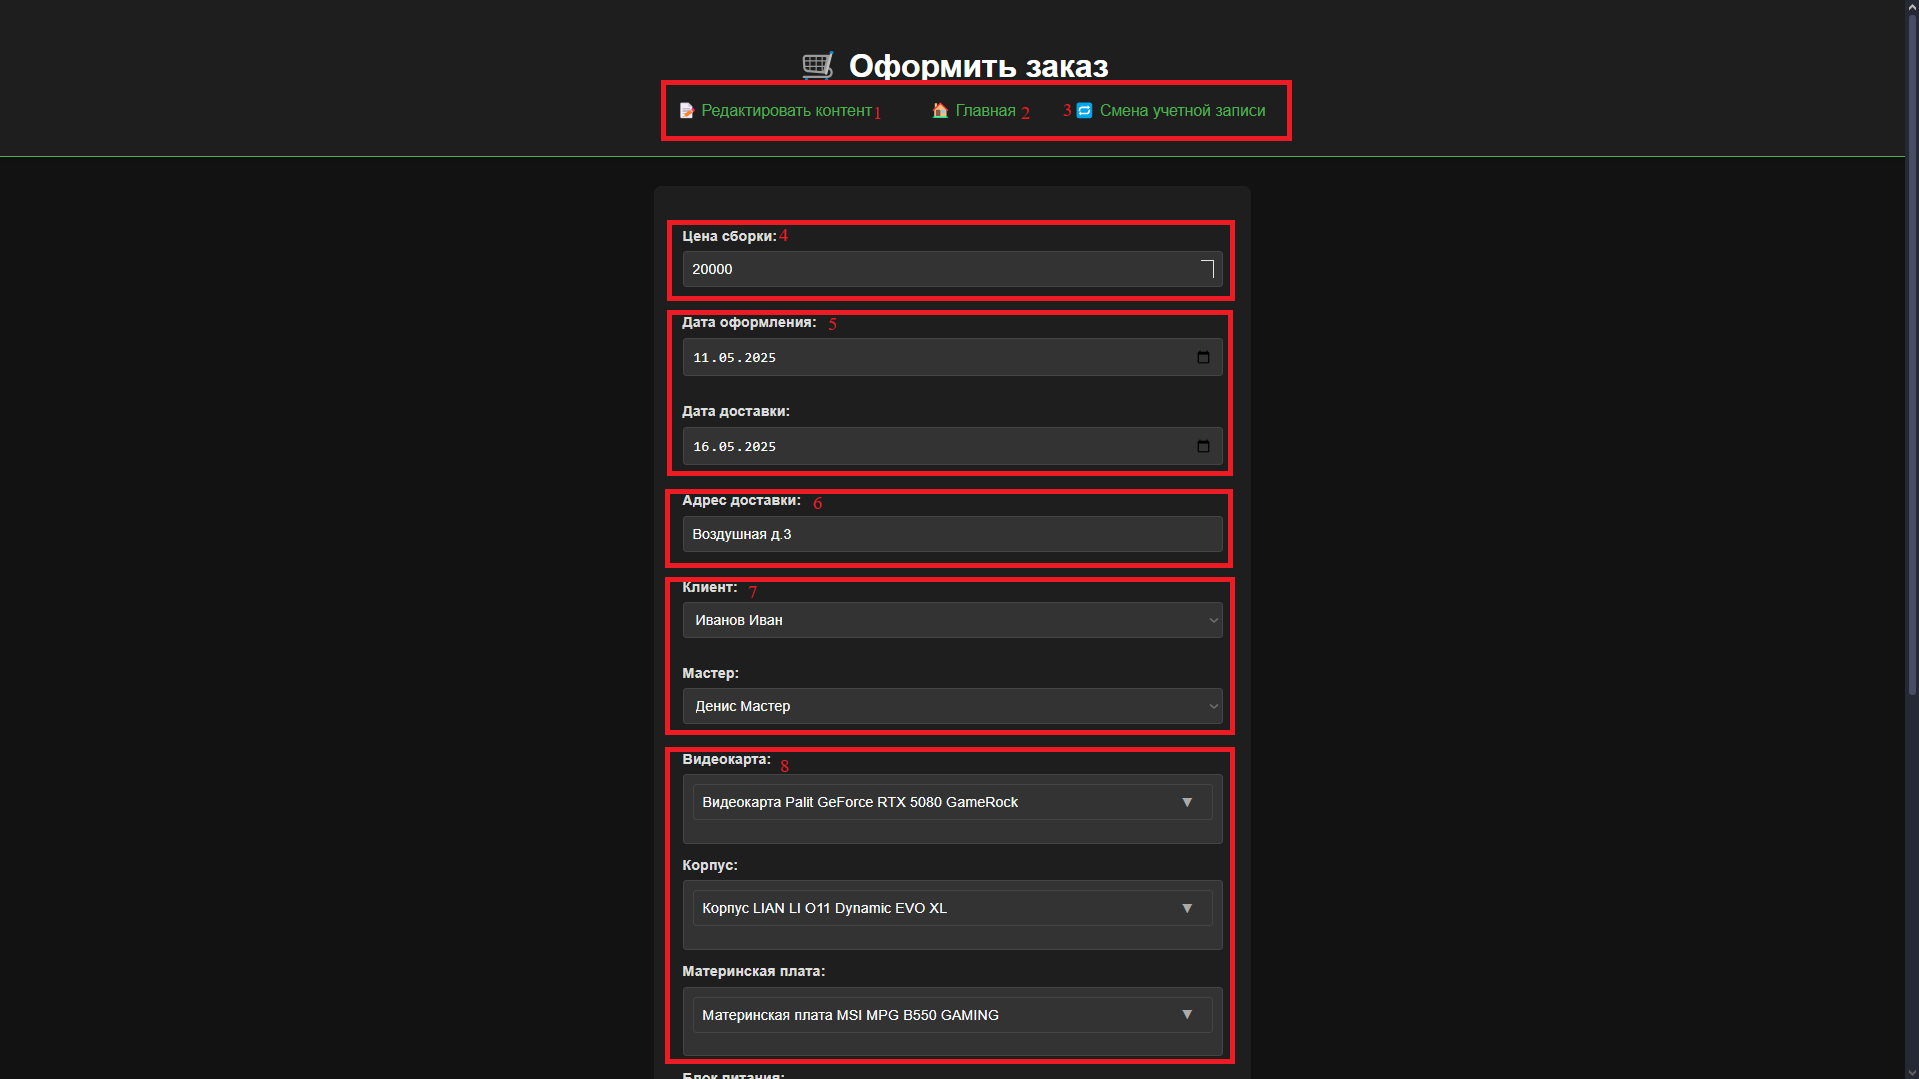
\includegraphics[width=0.9\linewidth]{order+fl}}
\center{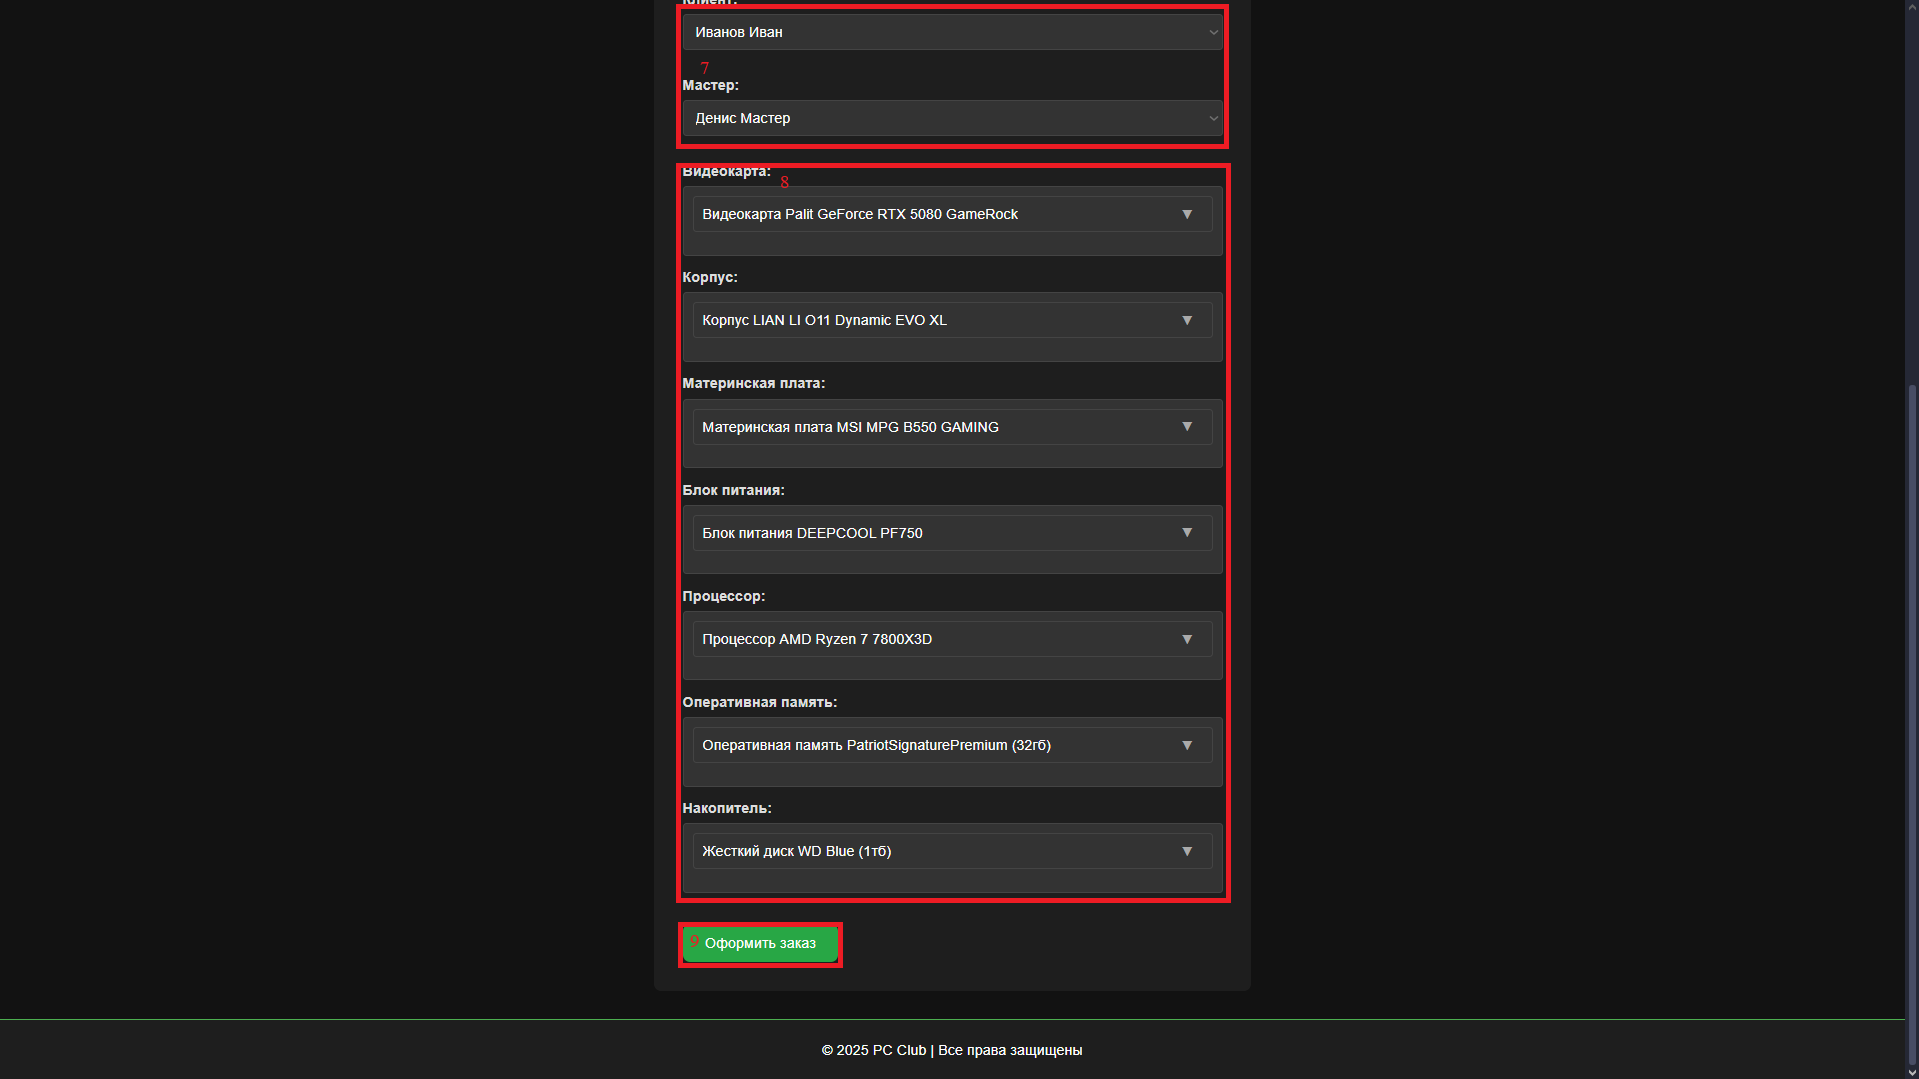
\includegraphics[width=0.9\linewidth]{order+fln}}
\center{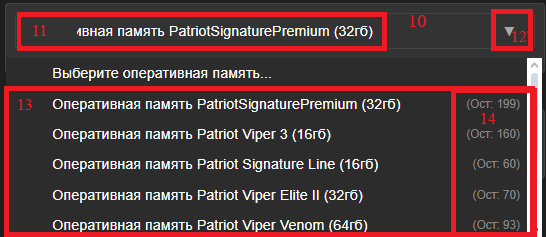
\includegraphics[width=0.75\linewidth]{chosenone}}
\caption{Страница оформления заказа и выпадающее меню компонента.}
\label{main:image}
\end{figure}

На рисунке \ref{login:image} меню для авторизации пользователей в системе, после авторизации под админской учетной записью можно получить доступ к админ панели, складу.
\begin{enumerate}
	\item Форма ввода логина.
	\item Форма ввода пароля.
	\item Кнопка сравнивает логин и хэш пароля с хранящимся в sql, при совпадении пропускает.
	\item Кнопка сохраняет логин и хэш пароля в sql.
	\item Вернуться на главную страницу.
\end{enumerate}
\begin{figure}[ht]
	\center{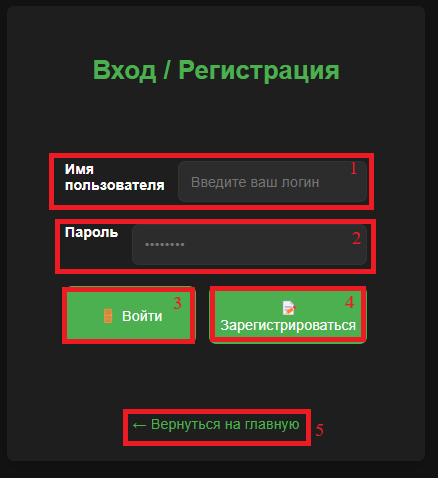
\includegraphics[width=0.25\linewidth]{login}}
	\caption{Разделы для каждого вида компонентов.}
	\label{login:image}
\end{figure}

На рисунке \ref{adminall:image} Панель администратора PC-Club позволяет полностью контролировать и редактировать информацию в sql.

\begin{enumerate}
	\item Панель навигации по сайту.
	\item Открыть меню выбора компонента.
	\item Ручной поиск по позициям и кнопка.
	\item Добавление новой записи в sql, через админ панель можно напрямую добавить новые компоненты в sql для их дальнейшего использования.
	\item Кнопка для редактирования, можно редактировать любую запись сделаную в таблицы sql.
	\item Кнопка для удаления, удалить любую запись из sql.
	\item Кнопка для экспорта данных таблицы заказа в файл.
	\item Заголовок таблицы, в нашем случае для заказов.
	\item Контент таблицы, хранимый и извлеченный из sql.
\end{enumerate}

\begin{figure}[ht]
\center{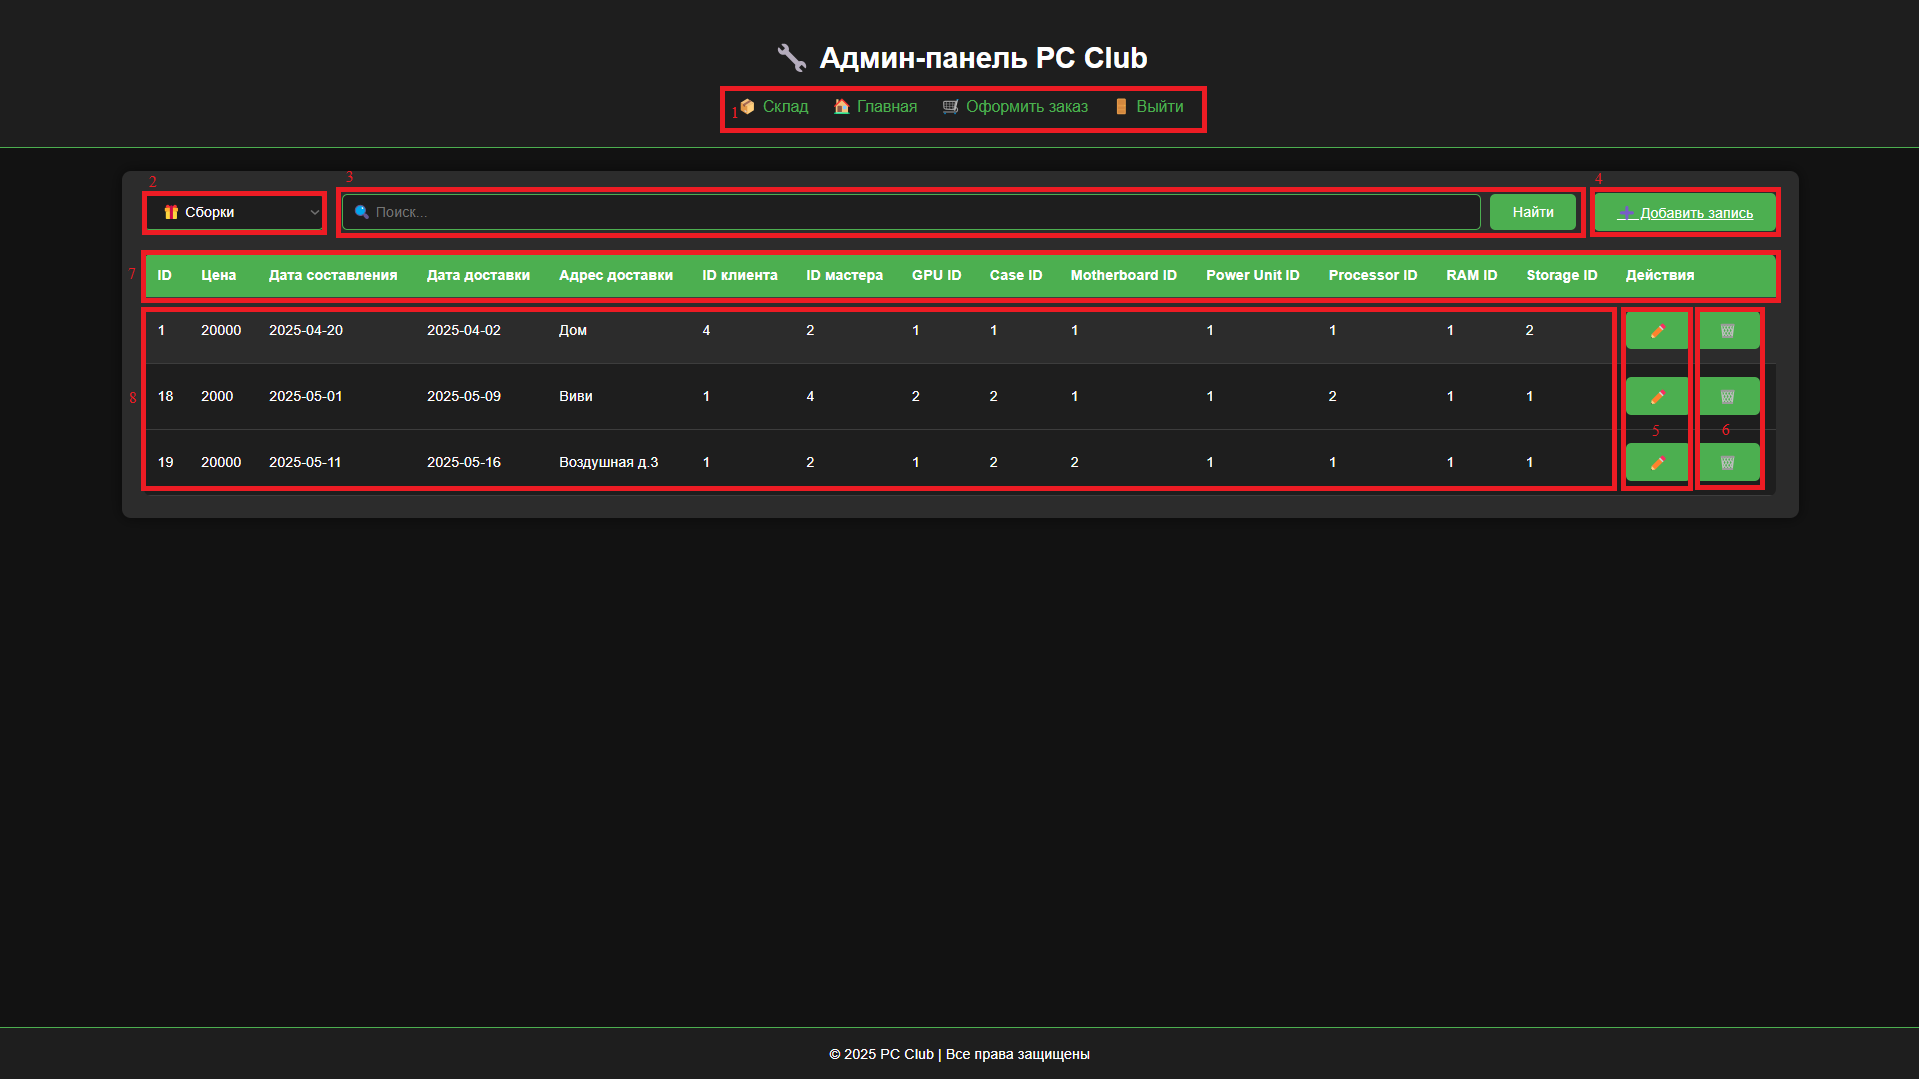
\includegraphics[width=1\linewidth]{adminall}}
\caption{Админ-панель PC-Club общий вид}
\label{adminall:image}
\end{figure}

На рисунке \ref{razdeli:image} меню выбора между типом компонентов в панели админа.

\begin{figure}[htbp]
\center{
\includegraphics[width=0.25\linewidth]{razdeli}}
\caption{Разделы для каждого вида компонентов.}
\label{razdeli:image}
\end{figure}

На рисунке \ref{storedf:image} меню менеджмента склада для веб-приложения, здесь можно пополнять запасы недостающих комплектующих, потом применять их в заказах.

\begin{enumerate}
	\item Расширенная навигационная панель админа.
	\item Кнопка вызова меню выбора типа компонента.
	\item Ручной поиск по позициям и кнопка.
	\item Заголовок таблицы.
	\item Компонент из таблицы.
	\item Количество компонента на складе и поле для ввода нового значения.
	\item Кнопка для обновления значения.
\end{enumerate}

\begin{figure}[ht]
	\center{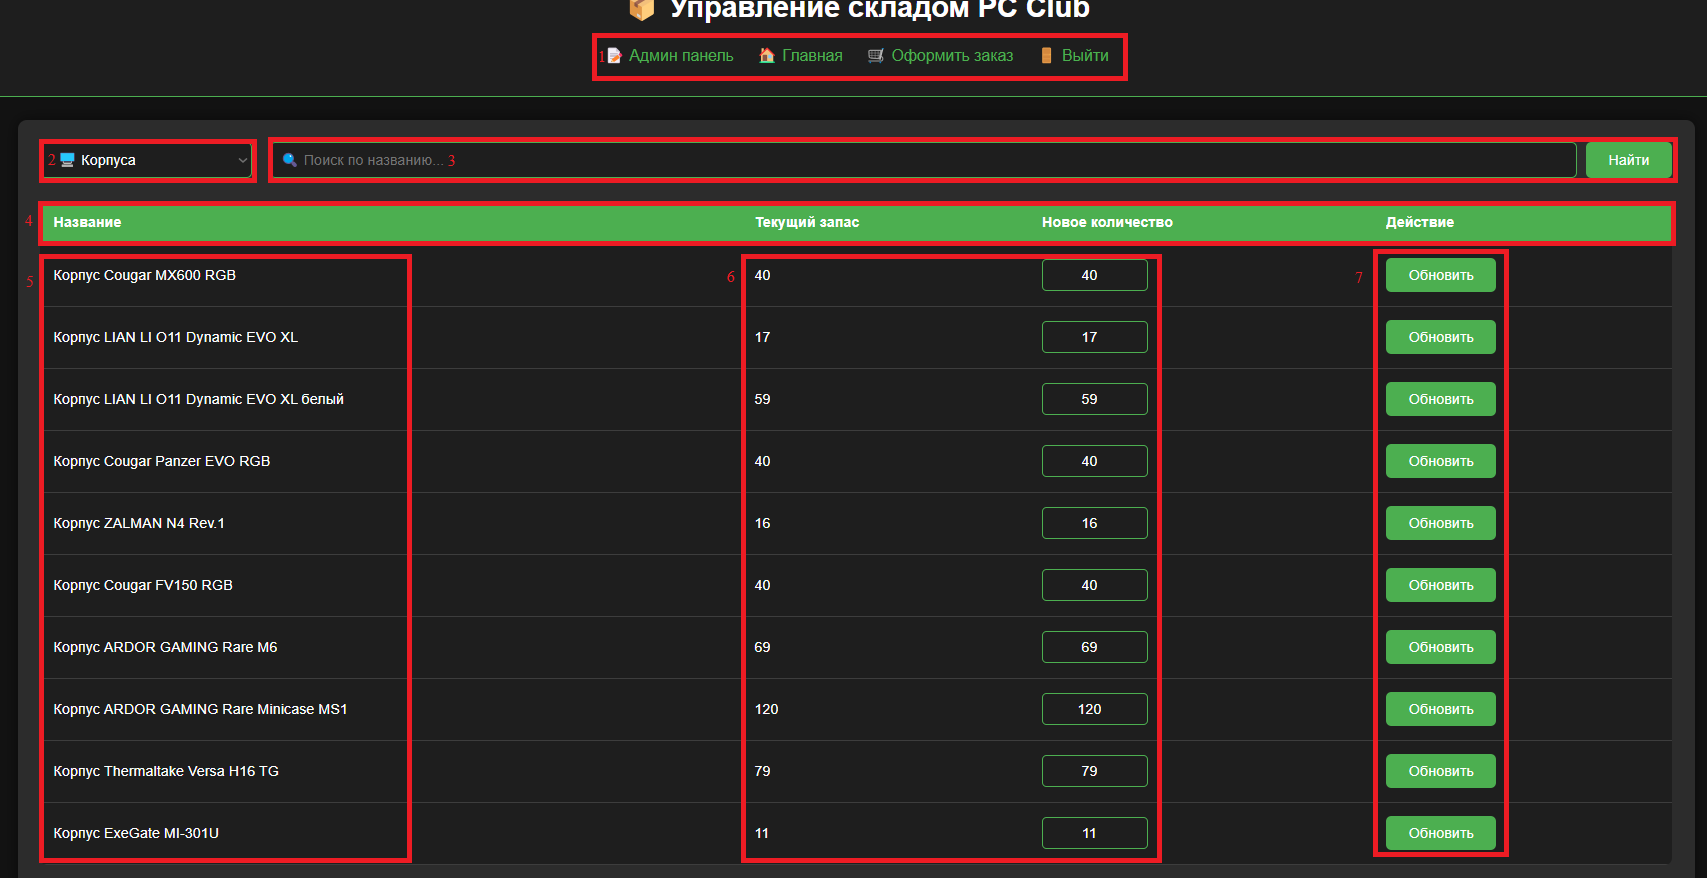
\includegraphics[width=1\linewidth]{storedf}}
	\caption{Страничка склада корпусов в качестве примера.}
	\label{storedf:image}
\end{figure}

\subsection{Тестирование программной системы}
Целью данного тестирования является проверка функциональности, надежности и производительности программно-информационной системы для управления сервис-центром.
Системное тестирование позволяет выявить и устранить ошибки, а также оценить соответствие системы предъявленным требованиям.

Все тестовые сценарии должны быть выполнены успешно без критических ошибок. Система должна обеспечивать стабильную работу и удобство использования в рамках установленных бизнес-процессов. Результаты тестирования будут использованы для повышения качества и надежности программного продукта.

\textbf{1) Запуск системы}

Описание: Система должна запускаться без ошибок и отображать главное окно интерфейса.

На рисунке ~\ref{storedf:index0} отображен успешный запуск системы и открытая главная страница.

\begin{figure}[ht]
	\center{
\includegraphics[width=1\linewidth]{index0}}
	\caption{Главная страница.}
	\label{storedf:index0}
\end{figure}

\textbf{2) Регистрация пользователя}

Описание: Пользователь должен иметь возможность создать новую учетную запись в системе.
Ожидаемый результат:  При вводе имени пользователя и пароля, нажатии на кнопку "Регистрация" пользователь создает новую запись в SQL. На рисунках \ref{storedf:login0}--\ref{storedf:loginc} тестируется регистрация нового пользователя. В то же время на рисунке ~\ref{storedf:login1} показан результат успешной регистрации пользователя в SQL. Пароль хэшируется для безопасного хранения данных пользователей.

\begin{figure}[ht]
	\center{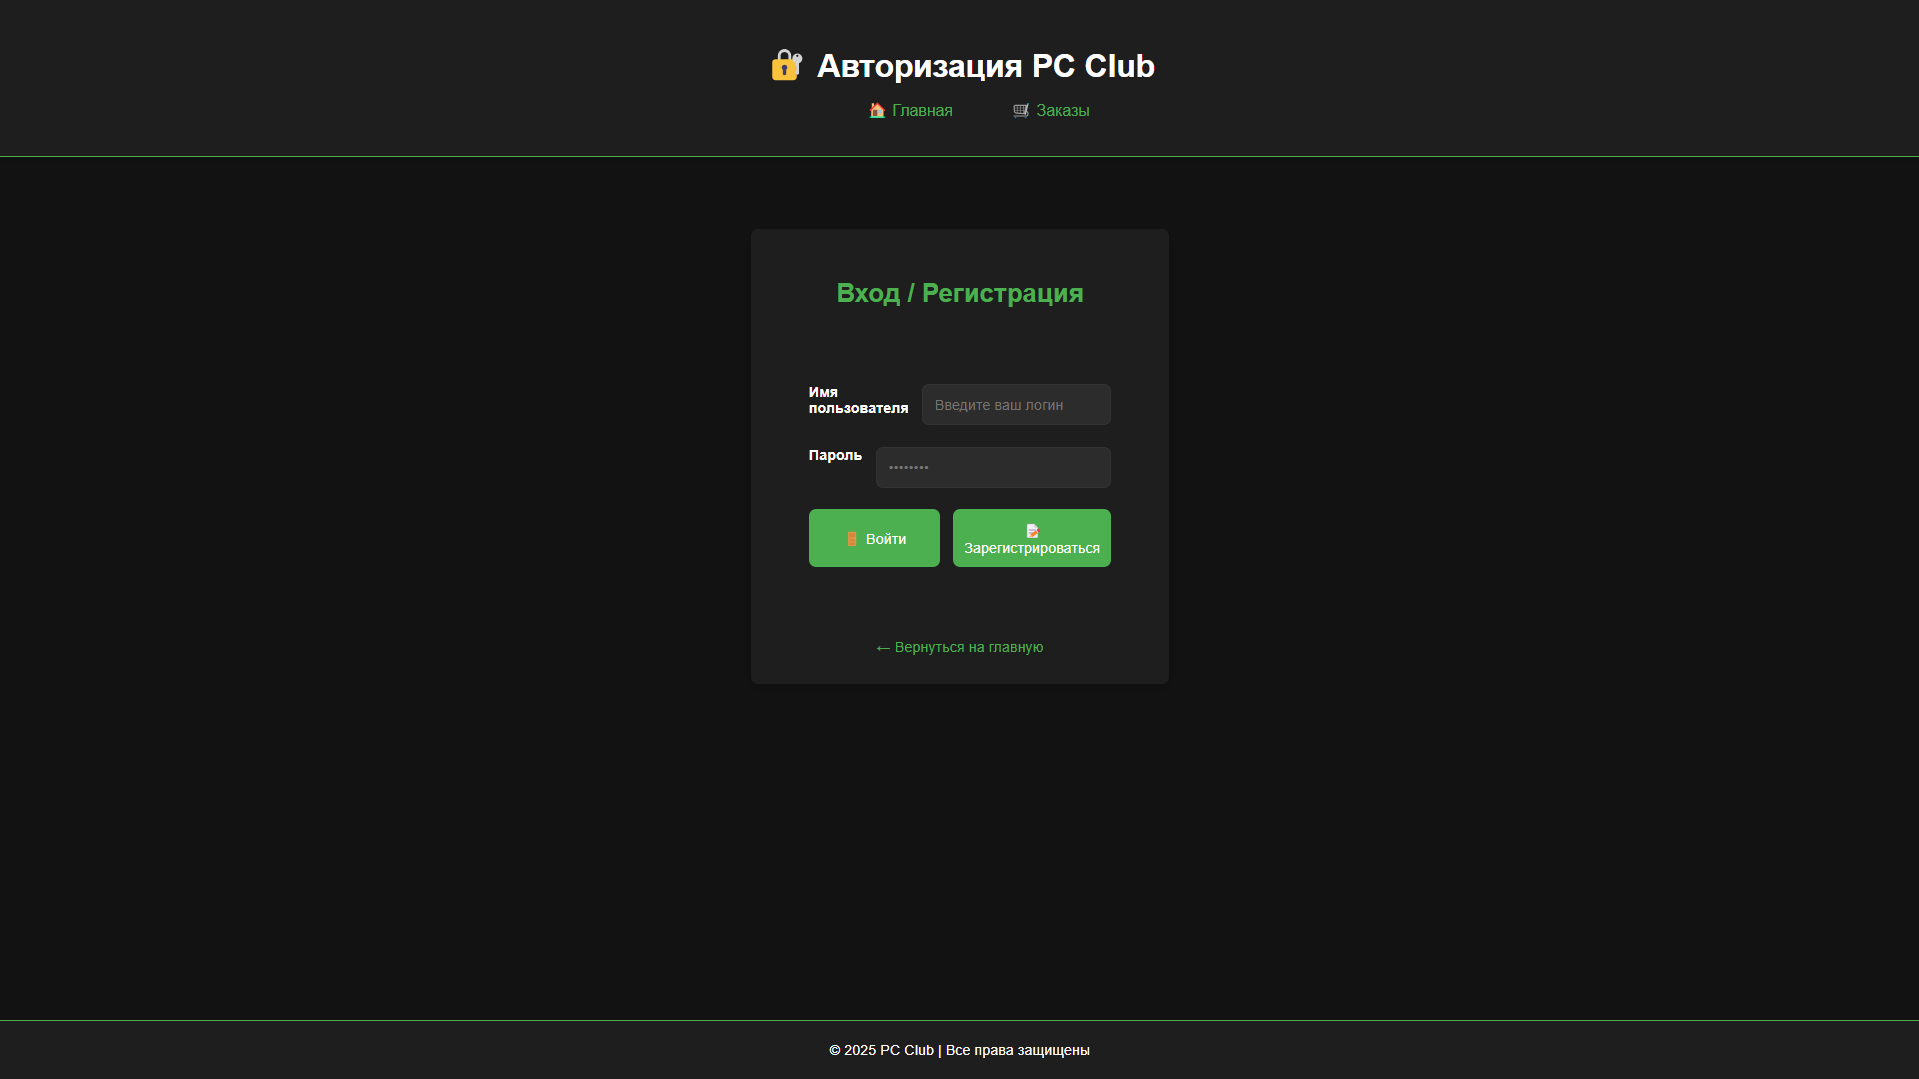
\includegraphics[width=1.0\linewidth]{login0}}
	\caption{Страница логин.}
	\label{storedf:login0}
\end{figure}

\begin{figure}[ht]
	\center{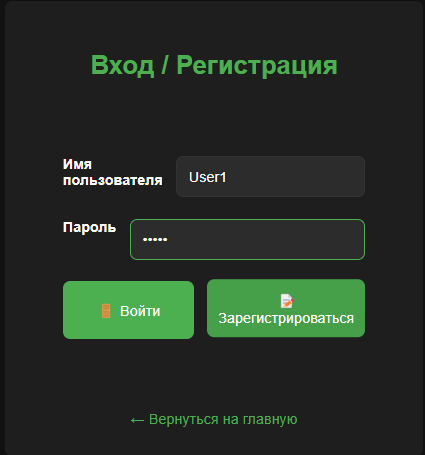
\includegraphics[width=0.6\linewidth]{loginus}}
	\caption{Регистрация.}
	\label{storedf:loginus}
\end{figure}

\begin{figure}[ht]
	\center{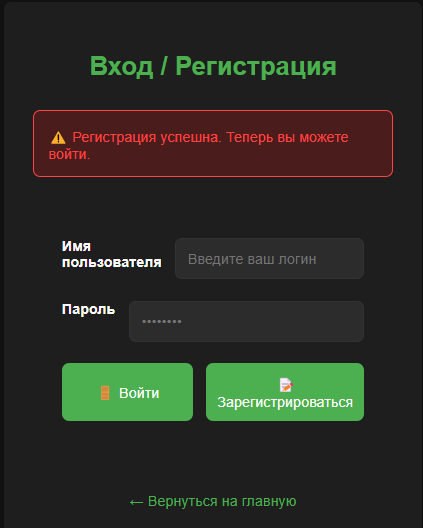
\includegraphics[width=0.6\linewidth]{loginc}}
	\caption{Результат регистрации.}
	\label{storedf:loginc}
\end{figure}

\begin{figure}[ht]
	\center{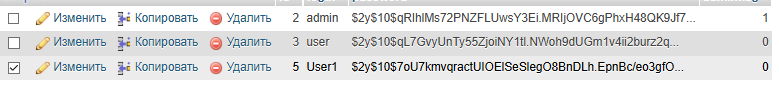
\includegraphics[width=1\linewidth]{login1}}
	\caption{Результат регистрации в SQL.}
	\label{storedf:login1}
\end{figure}


\clearpage 

\textbf{2) Авторизация пользователя}

Описание: Пользователь должен иметь возможность войти в свою учетную запись используя корректные имя пользователя и пароль.
Ожидаемый результат: Пользователь входит в свою учетную запись и получает доступ к своим функциям, пример на рисунках \ref{storedf:loginad}--\ref{storedf:panel0}.

\begin{figure}[ht]
	\center{
\includegraphics[width=0.5\linewidth]{loginad}}
	\caption{Окно авторизации.}
	\label{storedf:loginad}
\end{figure}

\begin{figure}[ht]
	\center{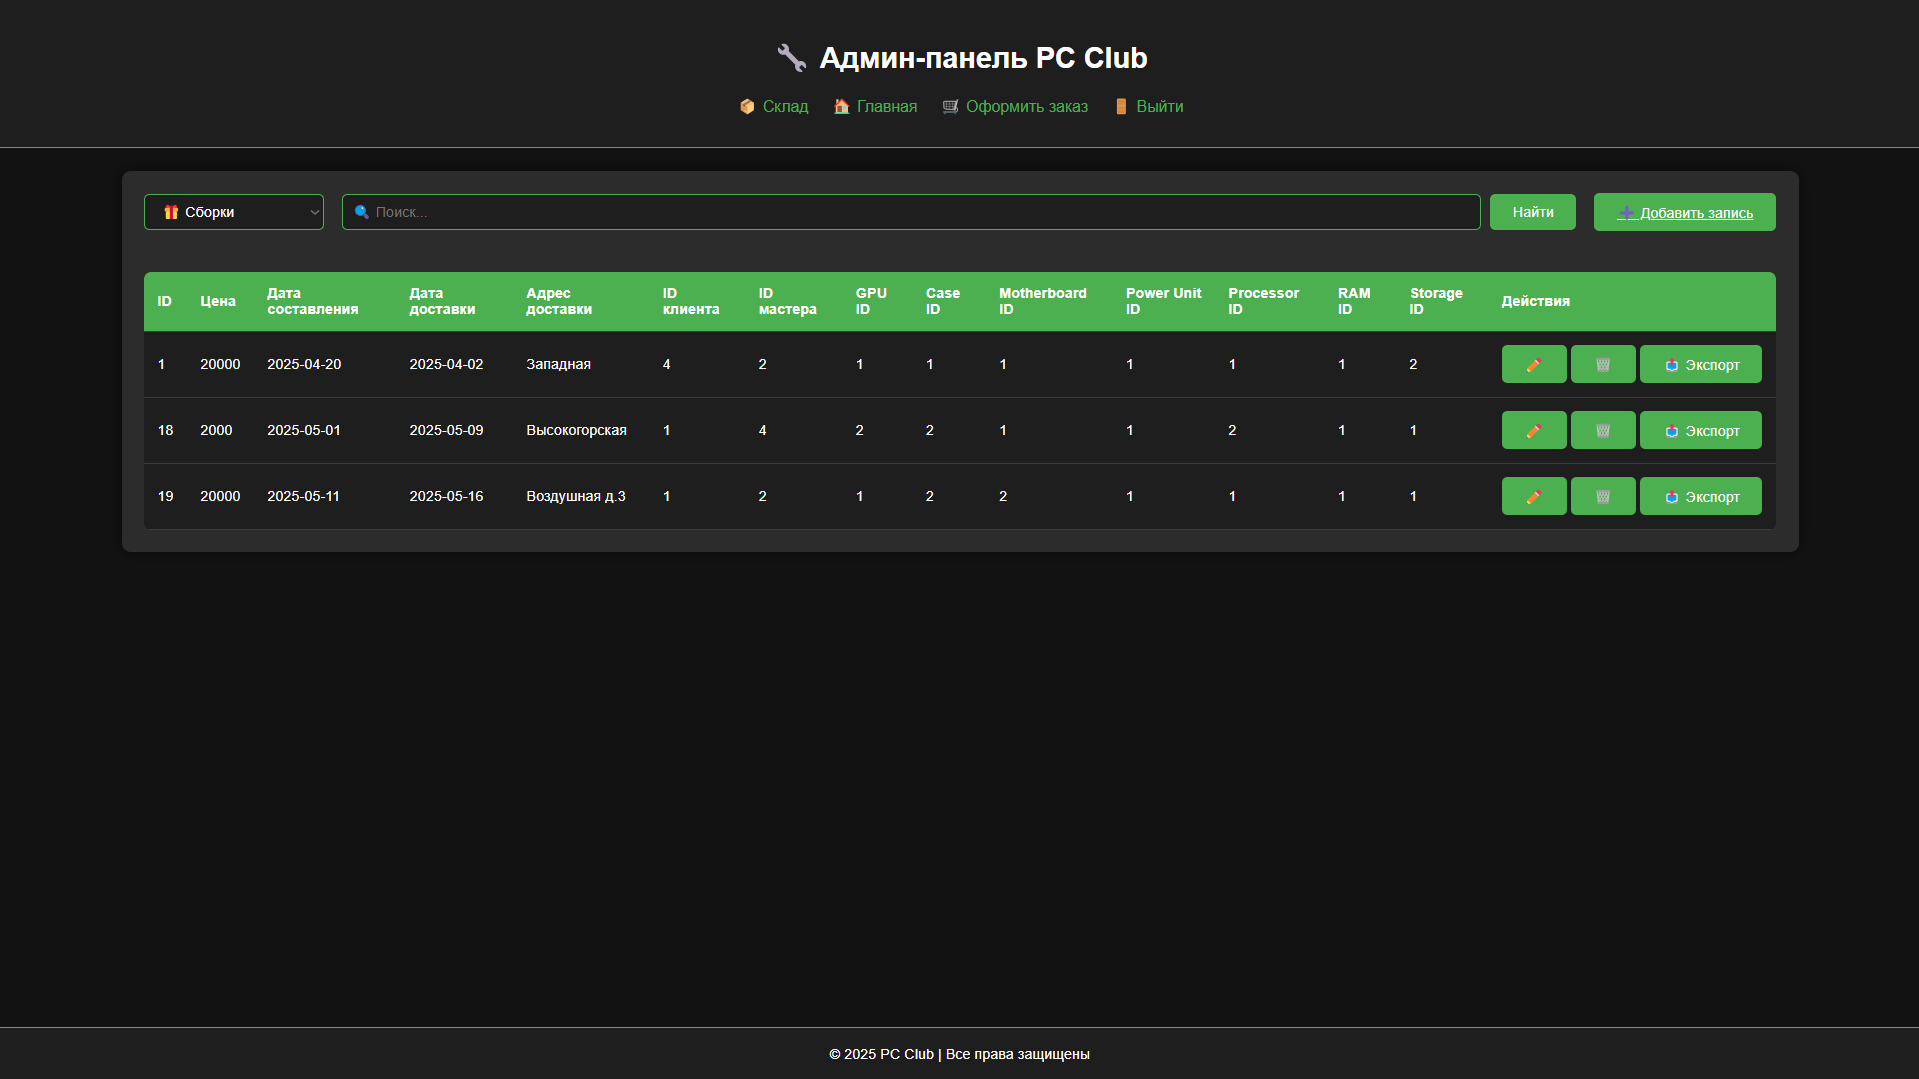
\includegraphics[width=0.9\linewidth]{panel0}}
	\caption{Результат авторизации пользователя.}
	\label{storedf:panel0}
\end{figure}

\textbf{3) Оформление заказа}

Описание: Пользователь должен иметь возможность создать новый заказ в системе.
Ожидаемый результат:  При вводе всех данных корректно отправляет новый заказ в систему.
На рисунках \ref{storedf:form0}--\ref{storedf:formgg1} отображен полный процесс оформления заказа и продемонстрировано появление новой записи в SQL.
\begin{figure}[ht]
	\center{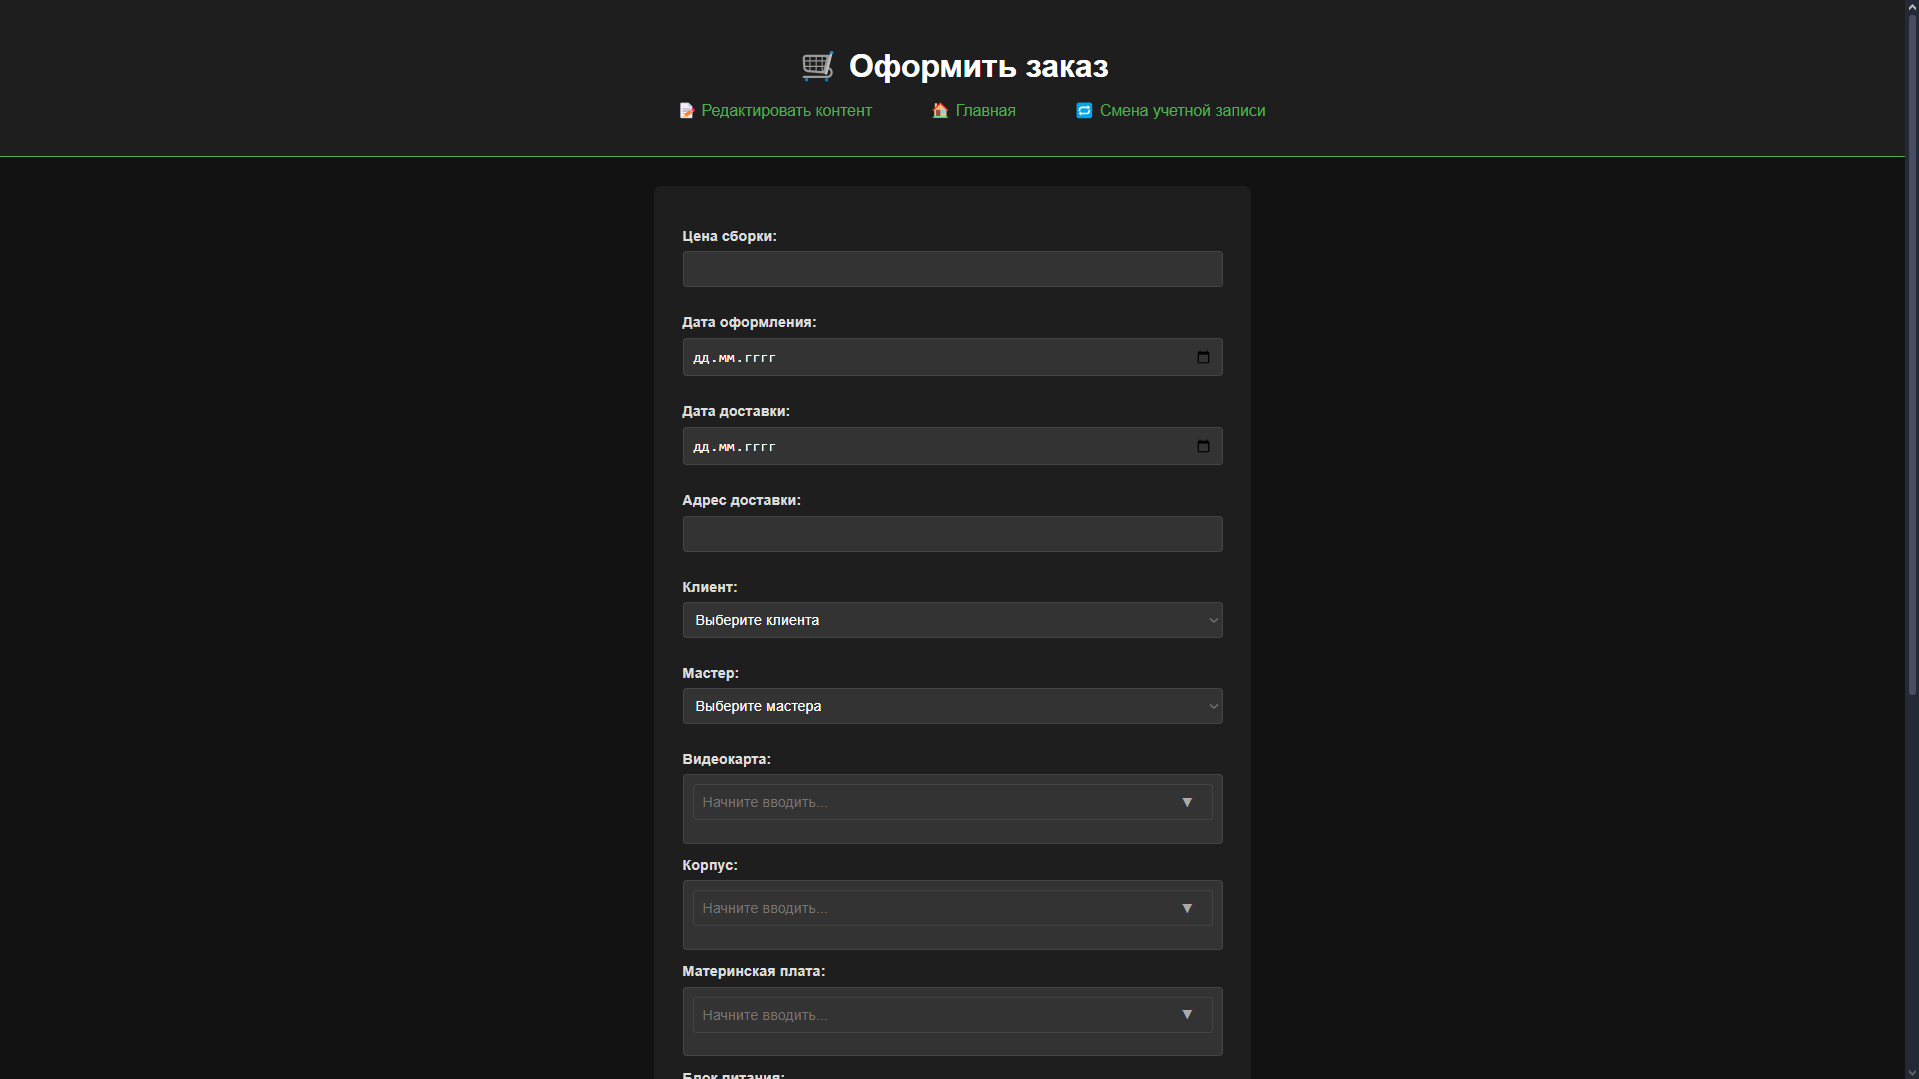
\includegraphics[width=0.9\linewidth]{form0}}
	\caption{Окно оформления заказа.}
	\label{storedf:form0}
\end{figure}

\begin{figure}[ht]
	\center{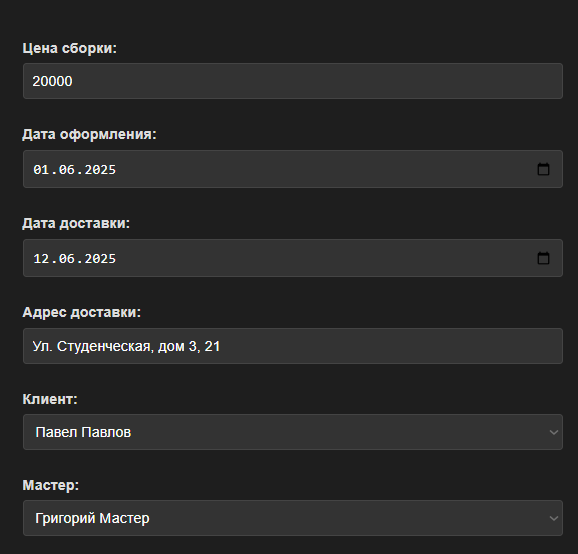
\includegraphics[width=0.5\linewidth]{form1}}
	\caption{Ввод данных заказа.}
	\label{storedf:form1}
\end{figure}

\begin{figure}[ht]
	\center{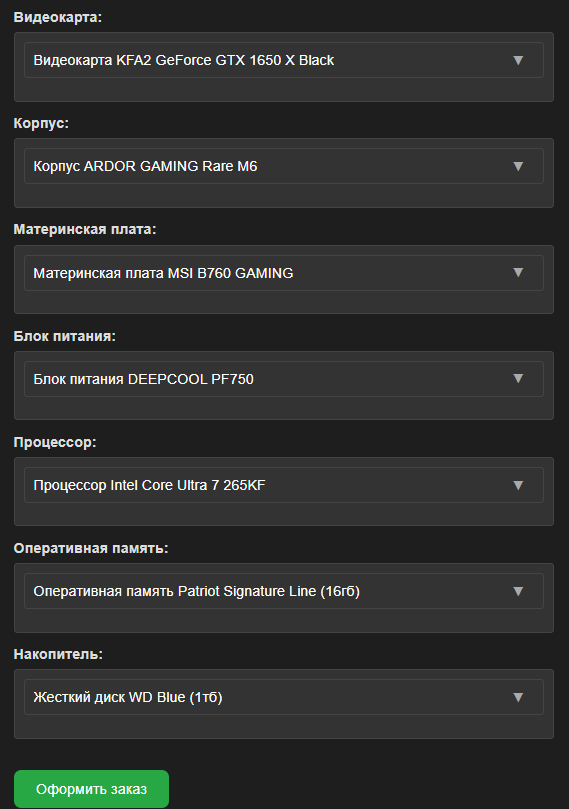
\includegraphics[width=0.5\linewidth]{form2}}
	\caption{Ввод технических данных компонентов заказа.}
	\label{storedf:form2}
\end{figure}

\begin{figure}[ht]
	\center{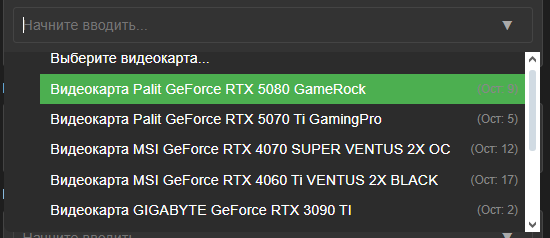
\includegraphics[width=1\linewidth]{formsearch0}}
	\caption{Селектор компонентов.}
	\label{storedf:formsearch0}
\end{figure}

\begin{figure}[ht]
	\center{
\includegraphics[width=1\linewidth]{formsearch1}}
	\caption{Результат поиска в селекторе.}
	\label{storedf:formsearch1}
\end{figure}

\begin{figure}[ht]
	\center{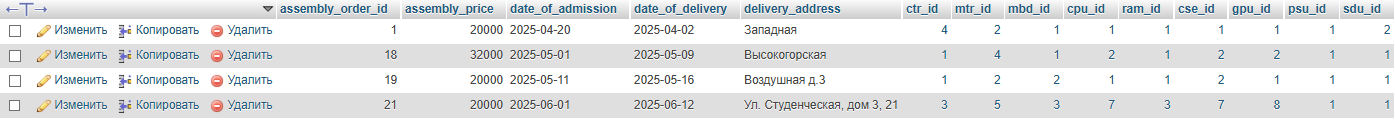
\includegraphics[width=1\linewidth]{formgg1}}
	\caption{Результат оформления заказа в SQL.}
	\label{storedf:formgg1}
\end{figure}

\newpage
\textbf{4) Отображение панели администратора}

Описание: Пользователь авторизован как администратор, панель администратора должна отображаться без ошибок. 

На рисунке \ref{storedf:panel0_} показан успешный вход в панель администратора.
\begin{figure}[ht]
	\center{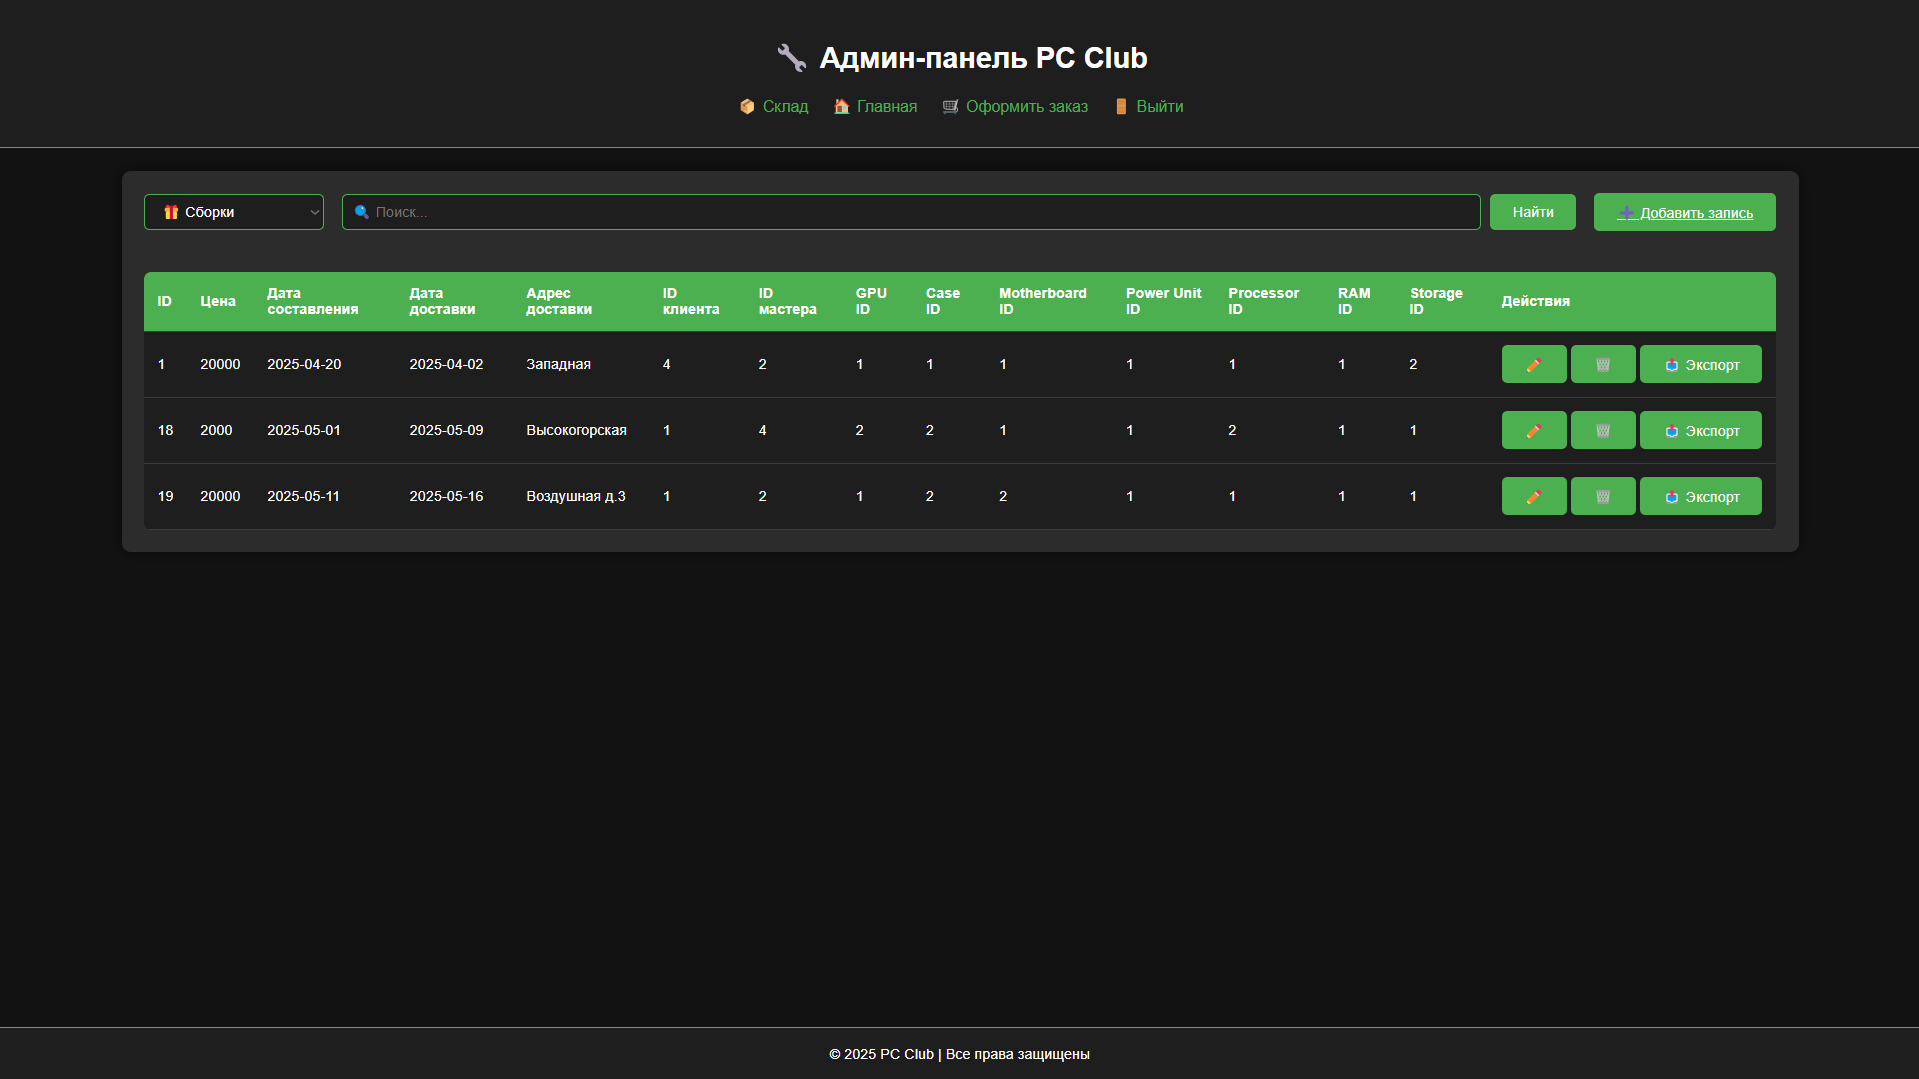
\includegraphics[width=0.9\linewidth]{panel0}}
	\caption{Отображение рабочей панели администратора.}
	\label{storedf:panel0_}
\end{figure}

\textbf{5) Редактирование данных записи}

На рисунках \ref{storedf:edit1}--\ref{stored:edit0} показано меню изменения записей.
\begin{enumerate}
\item Пользователь нажимает на кнопку "карандаш".
\item Меняет данные в заказе.
\item Сохраняет изменения.
\end{enumerate}

\begin{figure}[ht]
	\center{
\includegraphics[width=0.8\linewidth]{edit1}}
	\caption{Результат редактирования.}
	\label{storedf:edit1}
\end{figure}

\begin{figure}[ht]
	\center{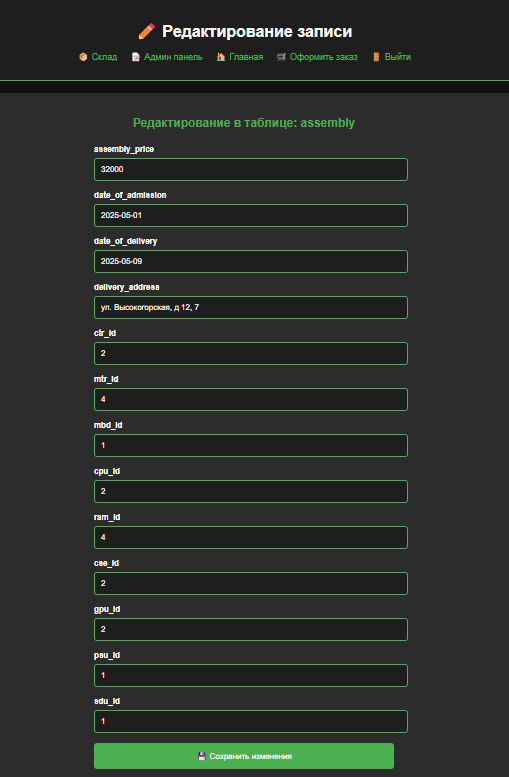
\includegraphics[width=0.74\linewidth]{edit0}}
	\caption{Интерфейс редактирования.}
	\label{stored:edit0}
\end{figure}

\textbf{6) Добавление новой записи}

На рисунках \ref{stored:addone}--\ref{stored:addone1} показано добавление новой записи в таблицу мастера.
\begin{enumerate}
	\item Пользователь нажимает на кнопку "добавить".
	\item Заполняет форму.
	\item Сохраняет запись.
\end{enumerate}

\begin{figure}[ht]
	\center{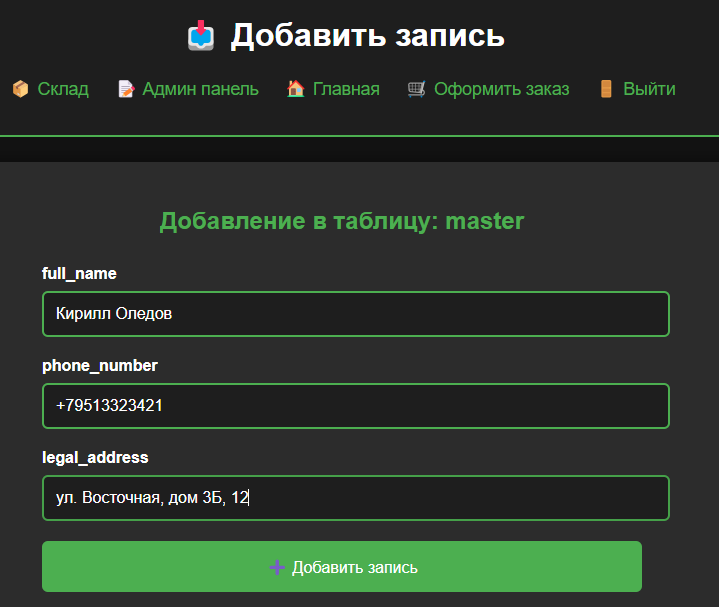
\includegraphics[width=0.7\linewidth]{addone}}
	\caption{Добавление новой записи.}
	\label{stored:addone}
\end{figure}

\begin{figure}[ht]
	\center{
\includegraphics[width=0.8\linewidth]{addone1}}
	\caption{Новая запись в системе.}
	\label{stored:addone1}
\end{figure}

\textbf{7) Удаление записи}

На рисунке \ref{stored:delete} показано окно подтверждения удаления записи из таблицы.
\begin{enumerate}
	\item Пользователь нажимает на кнопку "удалить".
	\item Подтверждает удаление.
\end{enumerate}

\begin{figure}[ht]
	\center{
\includegraphics[width=0.5\linewidth]{delete}}
	\caption{Новая запись в системе.}
	\label{stored:delete}
\end{figure}
\newpage

\textbf{8) Экспорт заказа в файл}

На рисунке \ref{stored:docdoc} показано содержимое .doc файла с экспортированной информацией.
\begin{enumerate}
	\item Пользователь нажимает на кнопку "экспорт".
	\item Пользователь получает файл с информацией о заказе.
\end{enumerate}

\begin{figure}[ht]
	\center{
\includegraphics[width=0.8\linewidth]{docdoc}}
	\caption{Сгенерированный .doc файл, содержит информацию о заказе.}
	\label{stored:docdoc}
\end{figure}

\textbf{9) Редактирование количества компонентов на складе}
Описание: Пользователь должен иметь возможность редактировать количество компонентов на складе.

Ожидаемый результат: На рисунках \ref{stored:warehouse0}--\ref{stored:stock2} пользователь редактирует количество компонентов.

\begin{figure}[ht]
	\center{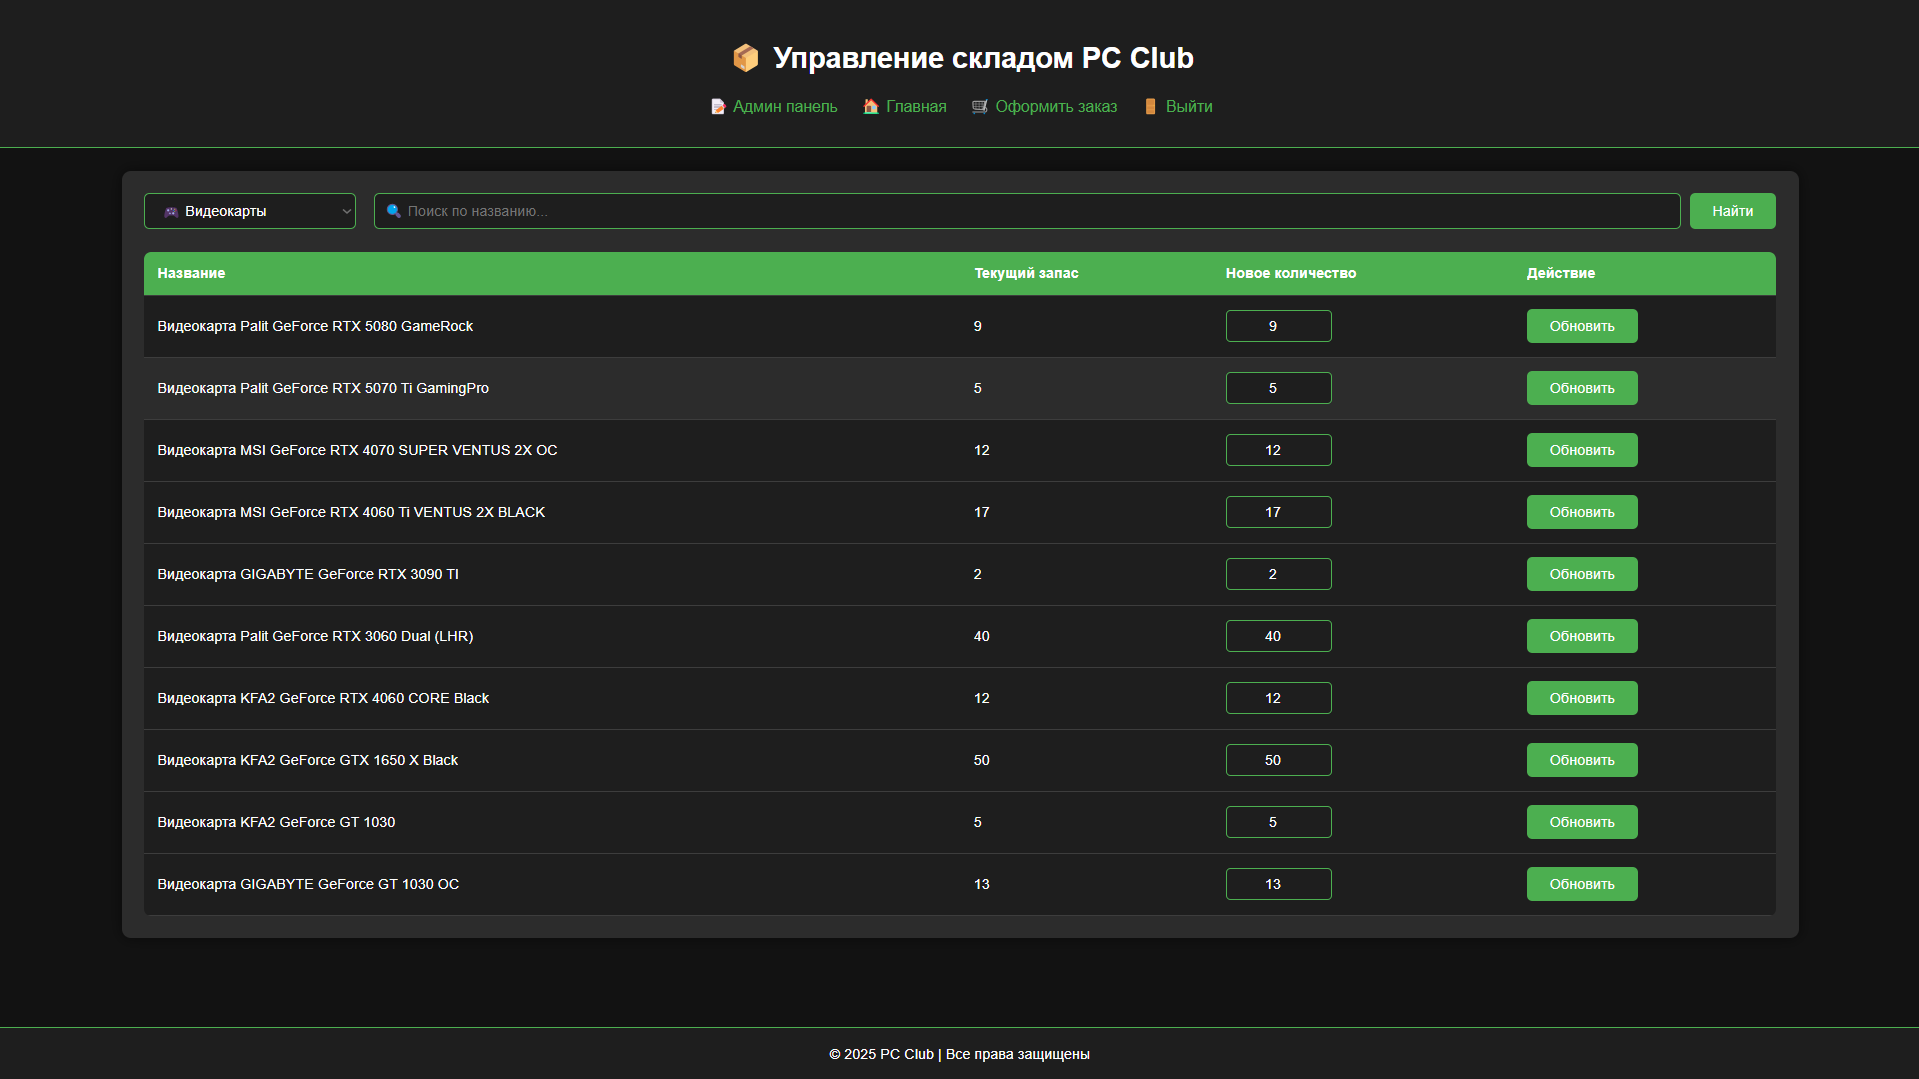
\includegraphics[width=1\linewidth]{warehouse0}}
	\caption{Окно с количеством компонентов на складе.}
	\label{stored:warehouse0}
\end{figure}

\begin{figure}[ht]
	\center{
\includegraphics[width=1\linewidth]{stock0}}
	\caption{Добавляем новое количество компонента.}
	\label{stored:stock0}
\end{figure}

\begin{figure}[ht]
	\center{
\includegraphics[width=1\linewidth]{stock1}}
	\caption{Уведомление об успехе.}
	\label{stored:stock1}
\end{figure}

\begin{figure}[ht]
	\center{
\includegraphics[width=1\linewidth]{stock2}}
	\caption{Обновленное количество компонента.}
	\label{stored:stock2}
\end{figure}

\clearpage
		\section*{ЗАКЛЮЧЕНИЕ}
\addcontentsline{toc}{section}{ЗАКЛЮЧЕНИЕ}

Разработанная программно-информационная система для сервисного центра «PC-Club» существенно повышает эффективность и качество обслуживания клиентов за счёт комплексной автоматизации ключевых бизнес-процессов и цифровизации взаимодействия между сотрудниками и посетителями. Внедрение системы обеспечивает удобство работы персонала, оптимизирует управление заказами и складскими запасами, а также улучшает коммуникацию с клиентами, что способствует росту числа заказчиков и укреплению конкурентных позиций компании на рынке.

В ходе работы были достигнуты следующие основные результаты:

\begin{enumerate}
	\item Проведен детальный анализ предметной области сервисного центра «PC-Club», включающий специфику ремонта персональных компьютеров, управление складом комплектующих и взаимодействие с клиентами. Для определения требований к системе изучены и проанализированы семь существующих программных продуктов, таких как RemOnline и HelloClient, выявлены их преимущества и недостатки.
	
	\item Разработана концептуальная модель программно-информационной системы, включающая архитектуру веб-приложения, построенную на основе UML-диаграмм прецедентов и компонентов, а также реляционную модель базы данных. Определены основные сущности системы: клиенты, заказы, комплектующие ПК, а также пользователи с разграничением ролей (администратор, клиент).
	
	\item Осуществлено проектирование трёхуровневой архитектуры системы с использованием технологий HTML, PHP и MySQL. Разработан удобный пользовательский интерфейс, включающий пять ключевых страниц: главная, оформление заказов, авторизация, админ-панель и управление складом. Внедрены механизмы безопасности, такие как хеширование паролей, защита от SQL-инъекций с помощью подготовленных запросов и валидация вводимых данных.
	
	\item Реализована и протестирована программно-информационная система с функционалом CRUD-операций для заказов и комплектующих, возможностью отслеживания остатков на складе в реальном времени, экспортом заказов в .doc-файлы и разделением прав доступа между администраторами и клиентами. Проведено системное тестирование, подтвердившее полное соответствие требованиям технического задания.
	
\end{enumerate}

Все требования, объявленные в техническом задании, были полностью реализованы, все задачи, поставленные в начале разработки проекта, были также решены.

Готовый рабочий проект представляет собой программно-информационную систему из серверной части, SQL и веб-приложения.
	}\fi
	\addcontentsline{toc}{section}{СПИСОК ИСПОЛЬЗОВАННЫХ ИСТОЧНИКОВ}

\begin{thebibliography}{9}

    \bibitem{javascript} 
    Абрамов, С. А. Методы оптимизации / С. А. Абрамов. – Москва: Наука, 1978. – 272 с. – Текст : непосредственный.
    
     \bibitem{javascript} 
    Васильев, В. И. Информационные системы / В. И. Васильев. – Москва: Финансы и статистика, 2009. – 416 с. – ISBN 978-5-279-03153-4. – Текст : непосредственный.
    
    \bibitem{javascript} 
    Гамзатов, М. Г. Информационные технологии / М. Г. Гамзатов, И. Г. Ахмедов. – Москва: Юрайт, 2018. – 392 с. – ISBN 978-5-534-05640-2. – Текст : непосредственный.
    
    \bibitem{javascript} 
    Голицына, О. Л. Информационные системы / О. Л. Голицына, Н. В. Максимов, И. И. Попов. – Москва: Форум, 2008. – 496 с. – ISBN 978-5-91134-245-4. – Текст : непосредственный.
    
    \bibitem{javascript} 
    Дейт, К. Введение в системы баз данных / К. Дейт. – Москва: Вильямс, 2006. – 1328 с. – ISBN 5-8459-0788-8. – Текст : непосредственный.
    
    \bibitem{javascript} 
    Информационные технологии: учебник для вузов / под ред. Н. В. Макаровой. – Москва: Финансы и статистика, 2005. – 768 с. – ISBN 5-279-02207-8. – Текст : непосредственный.
    
    \bibitem{javascript} 
    Кнут, Д. Искусство программирования / Д. Кнут. – Москва: Вильямс, 2000. – Т. 1. – 720 с. – ISBN 5-8459-0080-8. – Текст : непосредственный.
    
    \bibitem{javascript} 
    Кузнецов, С. В. Базы данных: учебник / С. В. Кузнецов. – Москва: Академия, 2007. – 496 с. – ISBN 978-5-7695-2477-0. – Текст : непосредственный.
    
    \bibitem{javascript}
    Литвиненко, В. В. Разработка информационных систем / В. В. Литвиненко. – Москва: Юрайт, 2018. – 344 с. – ISBN 978-5-534-07421-5. – Текст : непосредственный.
    
    \bibitem{javascript}
    Маклаков, С. В. BPWin и ERWin. CASE-средства разработки информационных систем / С. В. Маклаков. – Москва: ДИАЛОГ-МИФИ, 2000. – 304 с. – ISBN 5-86404-090-3. – Текст : непосредственный.
    
    \bibitem{javascript}
    Мартин, Д. Организация баз данных в вычислительных системах / Д. Мартин. – Москва: Мир, 1980. – 662 с. – Текст : непосредственный.
    
    \bibitem{javascript}
    Новиков, Ф. А. Дискретная математика для программистов / Ф. А. Новиков. – Санкт-Петербург: Питер, 2000. – 304 с. – ISBN 5-272-00176-4. – Текст : непосредственный.
    
    \bibitem{javascript}
    Робертсон, С. Осваиваем SQL за 24 часа / С. Робертсон. – Москва: Вильямс, 2002. – 272 с. – ISBN 5-8459-0315-7. – Текст : непосредственный.
    
    \bibitem{javascript}
    Таненбаум, Э. Современные операционные системы / Э. Таненбаум. – Санкт-Петербург: Питер, 2002. – 1040 с. – ISBN 5-318-00299-4. – Текст : непосредственный.
    
    \bibitem{javascript}
    Титтел, Э. HTML5 и CSS3 для чайников / Э. Титтел, К. Минник. – Москва: Вильямс, 2016. – 400 с. – ISBN 978-1-118-65720-1. – Текст : непосредственный.
    
    \bibitem{javascript}
    Электронный ресурс]. – URL: http://www.website.com (дата обращения: 15.05.2023). – Текст : электронный.
    
    \bibitem{javascript}
    Иванов, И. И. Анализ предметной области [Электронный ресурс] / И. И. Иванов. – Режим доступа: URL: http://www.example.com/ivanov (дата обращения: 20.05.2023). – Текст : электронный.
    
    \bibitem{javascript}
    Петров, П. П. Разработка информационной системы [Электронный ресурс] / П. П. Петров. – Режим доступа: URL: http://www.example.com/petrov (дата обращения: 25.05.2023). – Текст : электронный.
    
    \bibitem{javascript}
    Сидоров, С. С. Тестирование программного обеспечения [Электронный ресурс] / С. С. Сидоров. – Режим доступа: URL: http://www.example.com/sidorov (дата обращения: 30.05.2023). – Текст : электронный.
    
    \bibitem{javascript}
    Смирнов, А. А. Введение в базы данных [Электронный ресурс] / А. А. Смирнов. – Режим доступа: URL: http://www.example.com/smirnov (дата обращения: 05.06.2023). – Текст : электронный.
\end{thebibliography}

	\ifВКР{\appendix{Представление графического материала}

Графический материал, выполненный на отдельных листах,
изображен на рисунках А.1--А.\arabic{числоПлакатов}.
\setcounter{числоПлакатов}{0}

\renewcommand{\thefigure}{А.\arabic{figure}} % шаблон номера для плакатов

\begin{landscape}

\begin{плакат}
    \includegraphics[width=0.82\linewidth,page=1]{plakati.pdf}
    \заголовок{Сведения о ВКРБ}
    \label{pl1:image}      
\end{плакат}

\begin{плакат}
	\includegraphics[width=0.82\linewidth,page=2]{plakati.pdf}
	\заголовок{Цели и задачи разработки}
	\label{pl2:image}      
\end{плакат}

\begin{плакат}
	\includegraphics[width=0.82\linewidth,page=3]{plakati.pdf}
	\заголовок{Концептуальная модель данных}
	\label{pl3:image}      
\end{плакат}

\begin{плакат}
	\includegraphics[width=0.82\linewidth,page=4]{plakati.pdf}
	\заголовок{Диаграмма прецедентов}
	\label{pl4:image}      
\end{плакат}

\begin{плакат}
	\includegraphics[width=0.82\linewidth,page=5]{plakati.pdf}
	\заголовок{Диаграмма компонентов}
	\label{pl5:image}      
\end{плакат}

\begin{плакат}
	\includegraphics[width=0.82\linewidth,page=6]{plakati.pdf}
	\заголовок{Страница регистрации и авторизации пользователей}
	\label{pl6:image}      
\end{плакат}

\begin{плакат}
	\includegraphics[width=0.82\linewidth,page=7]{plakati.pdf}
	\заголовок{Главная страница}
	\label{pl7:image}      
\end{плакат}

\begin{плакат}
	\includegraphics[width=0.82\linewidth,page=8]{plakati.pdf}
	\заголовок{Страница с панелью администратора}
	\label{pl8:image}      
\end{плакат}

\begin{плакат}
	\includegraphics[width=0.82\linewidth,page=9]{plakati.pdf}
	\заголовок{Страница для управления скалдом}
	\label{pl9:image}      
\end{плакат}

\begin{плакат}
	\includegraphics[width=0.82\linewidth,page=10]{plakati.pdf}
	\заголовок{Страница оформления заказов}
	\label{pl10:image}      
\end{плакат}

\begin{плакат}
	\includegraphics[width=0.82\linewidth,page=11]{plakati.pdf}
	\заголовок{Заключение}
	\label{pl11:image}      
\end{плакат}

\end{landscape}
}\fi
	\ifПрактика{}\else{\appendix{Фрагменты исходного кода программы}


Orderform.php
\begin{figure}[ht]
	\begin{lstlisting}[language=Php]
		// Функция получения компонентов и загрузка данных
		function getComponents($link, $table, $id_col, $name_col, $check_stock = false) {
			$data = [];
			$sql = $check_stock 
			? "SELECT $id_col, $name_col, stock FROM $table WHERE stock > 0"
			: "SELECT $id_col, $name_col FROM $table";
			
			$result = mysqli_query($link, $sql);
			if ($result && mysqli_num_rows($result) > 0) {
				while ($row = mysqli_fetch_assoc($result)) {
					$item = ['name' => $row[$name_col]];
					if ($check_stock) $item['stock'] = $row['stock'];
					$data[$row[$id_col]] = $item;
				}
			}
			return $data;
		}
		
		$customers = getComponents($link, 'customer', 'ctr_id', 'full_name');
		$masters = getComponents($link, 'master', 'mtr_id', 'full_name');
		
		$components = [
		'gpu' => getComponents($link, 'gpu', 'gpu_id', 'gpu_name', true),
		'mcase' => getComponents($link, 'mcase', 'cse_id', 'case_name', true),
		'motherboard' => getComponents($link, 'motherboard', 'mbd_id', 'motherboard_name', true),
		'powerunit' => getComponents($link, 'powerunit', 'psu_id', 'power_name', true),
		'processor' => getComponents($link, 'processor', 'cpu_id', 'unit_name', true),
		'ram' => getComponents($link, 'ram', 'ram_id', 'ram_name', true),
		'storage' => getComponents($link, 'storage', 'sdu_id', 'storage_name', true)
		];
	\end{lstlisting}
	\caption{Функция получения компонентов и загрузка данных}
	\label{fig:orderform_part1}
\end{figure}

\begin{figure}[ht]
	\begin{lstlisting}[language=Php]
		// Обработка POST-запроса и валидация данных
		$errors = [];
		$success_message = '';
		
		if ($_SERVER["REQUEST_METHOD"] == "POST") {
			// Валидация данных
			$assembly_price = $_POST["assembly_price"];
			if (strlen($assembly_price) > 6) {
				$errors['assembly_price'] = "Цена должна содержать не более 6 символов.";
			} elseif (!is_numeric($assembly_price) || $assembly_price < 0) {
				$errors['assembly_price'] = "Цена должна быть неотрицательным числом.";
			}
			
			$delivery_address = $_POST["delivery_address"];
			if (strlen($delivery_address) > 110) {
				$errors['delivery_address'] = "Адрес доставки не должен превышать 110 символов.";
			}
			
			$date_of_admission = $_POST["date_of_admission"];
			$date_of_delivery = $_POST["date_of_delivery"];
			
			if (strtotime($date_of_admission) > time()) {
				$errors['date_of_admission'] = "Дата оформления не может быть в будущем.";
			}
			
			if (strtotime($date_of_delivery) < strtotime($date_of_admission)) {
				$errors['date_of_delivery'] = "Дата доставки должна быть позже даты оформления.";
			}			
			$component_ids = [
			'gpu_id' => $_POST['gpu_id'],
			'cse_id' => $_POST['cse_id'],
			'mbd_id' => $_POST['mbd_id'],
			'psu_id' => $_POST['psu_id'],
			'cpu_id' => $_POST['cpu_id'],
			'ram_id' => $_POST['ram_id'],
			'sdu_id' => $_POST['sdu_id']
			];		
			.
			.
			.
			.
			.		   
	\end{lstlisting}
\caption{Обработка формы заказа и обновление базы данных}
\label{fig:orderform_part2}
\end{figure}

\begin{figure}[ht]
	\begin{lstlisting}[language=Php]
			if (empty($errors)) {
				mysqli_autocommit($link, false);				
				try {
					// Проверка остатков компонентов
					foreach ($component_ids as $field => $id) {
						$table = get_table_name($field);
						$stmt = $link->prepare("SELECT stock FROM $table WHERE ".get_id_column($table)." = ? FOR UPDATE");
						$stmt->bind_param("i", $id);
						$stmt->execute();
						$result = $stmt->get_result();						
						if (!$result || $result->num_rows === 0) {
							throw new Exception("Компонент $table не найден");
						}						
						$row = $result->fetch_assoc();
						if ($row['stock'] < 1) {
							throw new Exception("Недостаточно $table на складе");
						}}					
					// Добавление заказа
					$stmt = $link->prepare("INSERT INTO assembly (
					assembly_price, date_of_admission, date_of_delivery, delivery_address,
					ctr_id, mtr_id, gpu_id, cse_id, mbd_id, psu_id, cpu_id, ram_id, sdu_id
					) VALUES (?, ?, ?, ?, ?, ?, ?, ?, ?, ?, ?, ?, ?)");					
					$stmt->bind_param("dsssiiiiiiiii",
					$_POST['assembly_price'],
					$_POST['date_of_admission'],
					$_POST['date_of_delivery'],
					$_POST['delivery_address'],
					$_POST['ctr_id'],
					$_POST['mtr_id'],
					$_POST['gpu_id'],
					$_POST['cse_id'],
					$_POST['mbd_id'],
					$_POST['psu_id'],
					$_POST['cpu_id'],
					$_POST['ram_id'],
					$_POST['sdu_id']);	
					if (!$stmt->execute()) throw new Exception("Ошибка оформления: ".$stmt->error);
					// Обновление остатков
					foreach ($component_ids as $field => $id) {
						$table = get_table_name($field);
						$stmt = $link->prepare("UPDATE $table SET stock = stock - 1 WHERE ".get_id_column($table)." = ?");
						$stmt->bind_param("i", $id);
						if (!$stmt->execute()) throw new Exception("Ошибка обновления: ".$stmt->error);}
	\end{lstlisting}
\caption{Обработка формы заказа и обновление базы данных}
\label{fig:orderform_part3}
\end{figure}

\clearpage
\begin{center}
\textbf{Место для диска}
\end{center}
\fi
}\fi
\end{document}
